\documentclass[12pt,a4paper,oneside]{report}

% =================================================
% PACKAGES
% =================================================
\usepackage[utf8]{inputenc}
\usepackage[T1]{fontenc}
\usepackage[french]{babel}
\usepackage[a4paper,margin=2.5cm]{geometry}
\usepackage{setspace}
\usepackage{indentfirst}
\usepackage{titlesec}
\usepackage{fancyhdr}
\usepackage{tocloft}
\usepackage{graphicx}
\usepackage{float}
\usepackage{xcolor}
\usepackage{array}
\usepackage{longtable}
\usepackage{booktabs}
\usepackage{caption}
\usepackage{hyperref}
\usepackage{enumitem}
\usepackage{amsmath}
\usepackage{tabularx}
\usepackage{multirow}
\usepackage{tikz}

\graphicspath{{./}{./image_web/img/}{./figures/}{./diagrammes/}{./diagrammes mobile/}{./Diagrammes pfe/sprint 1/}{./Diagrammes pfe/sprint2/}{./Diagrammes pfe/sprint3/}{./Diagrammes pfe/sprint4/}{./Diagrammes pfe/sprint 5/}}
\setlength{\headheight}{15pt}
\addtolength{\topmargin}{-3pt}

\onehalfspacing
\setlength{\parskip}{0.3em}
\setlength{\parindent}{1.25em}

\hypersetup{
    colorlinks=true,
    linkcolor=black,
    urlcolor=blue,
    citecolor=black,
    pdftitle={Rapport de Projet de Fin d'Études},
    pdfauthor={Med Amine Ben Moussa}
}

% =================================================
% COMMANDE PLACEHOLDER IMAGE
% =================================================
\newcommand{\imgplaceholder}[3]{%
  \begin{tikzpicture}
    \draw[thick, dashed, gray] (0,0) rectangle (#1,#2);
    \node[gray, font=\small\itshape] at (#1/2, #2/2) {#3};
  \end{tikzpicture}%
}

% =================================================
% STYLE DES CHAPITRES
% =================================================
\titleformat{\chapter}[display]
  {\normalfont\bfseries\centering}
  {\Huge Chapitre \thechapter}
  {0.5em}
  {\LARGE}
\titlespacing*{\chapter}{0pt}{-10pt}{20pt}

% =================================================
% EN-TETE / PIED DE PAGE
% =================================================
\pagestyle{fancy}
\fancyhf{}
\fancyfoot[C]{\thepage}
\fancyhead[L]{\nouppercase{\leftmark}}
\renewcommand{\headrulewidth}{0.3pt}
\renewcommand{\footrulewidth}{0pt}

\newcommand{\HRule}{\rule{\linewidth}{0.5mm}}

\begin{document}

% =================================================
% PAGE DE GARDE
% =================================================
\begin{titlepage}
\thispagestyle{empty}
\begin{center}

\begin{minipage}{0.18\textwidth}
\raggedright
% \includegraphics[width=2.2cm]{Reseau-ISET.png}
\imgplaceholder{2.2cm}{2.2cm}{Reseau-ISET.png}
\end{minipage}
\begin{minipage}{0.58\textwidth}
\centering
{\small \textbf{Ministère de l'Enseignement Supérieur et de la Recherche Scientifique}}\\[0.1cm]
{\small \textbf{Direction Générale des Études Technologiques}}\\[0.1cm]
{\small \textbf{Institut Supérieur des Études Technologiques de Kélibia}}\\[0.1cm]
{\small \textbf{Département Technologie de l'Informatique}}
\end{minipage}
\begin{minipage}{0.18\textwidth}
\raggedleft
\includegraphics[width=2.2cm]{Logo_ISET_Kelibia.jpg}
\end{minipage}

\vspace{1cm}
{\Large Rapport de Projet de Fin d'Études}\\[0.8cm]
{\normalsize Élaboré par : Med Amine Ben Moussa}\\[0.6cm]
\rule{0.75\textwidth}{0.5pt}\\[0.5cm]
{\Large \textbf{Développement d'un Système de Gestion des}}\\[0.15cm]
{\Large \textbf{Ordres de Transports -- OTFLOW}}\\[0.5cm]
\rule{0.75\textwidth}{0.5pt}\\[0.8cm]
{\normalsize Réalisé au sein de : Lumière Transport}\\[0.4cm]
\includegraphics[width=4cm]{lumiere.png}\\[0.8cm]
{\normalsize Encadré par :}\\[0.4cm]
{\small Encadrant industriel : M. Hakim Ben Chikh}\\[0.2cm]
{\small Encadrant académique : Mme Houda Toukabri}\\[0.8cm]
{\normalsize \textbf{Année universitaire 2025 / 2026}}

\end{center}
\end{titlepage}

% =================================================
% PARTIE PRELIMINAIRE
% =================================================
\pagenumbering{roman}
\setcounter{page}{1}

% -------------------------------------------------
\chapter*{Dédicace}
\addcontentsline{toc}{chapter}{Dédicace}
\vspace{1cm}
\textit{À compléter.}

% -------------------------------------------------
\chapter*{Remerciements}
\addcontentsline{toc}{chapter}{Remerciements}

Au terme de ce Projet de Fin d'Études, je tiens à exprimer ma profonde gratitude envers toutes les personnes qui ont contribué à la réussite de ce travail.

Je remercie l'entreprise Lumière Transports pour m'avoir accueilli et offert l'opportunité de réaliser ce projet dans un environnement professionnel enrichissant. J'exprime ma gratitude à mon encadrant industriel, M. Hakim Ben Chikh, dont les orientations et l'expertise métier ont été un guide essentiel. Mes sincères remerciements vont également à mon encadrant académique, Mme Houda Toukabri, pour son encadrement méthodologique et son soutien continu. Enfin, je remercie l'ensemble des enseignants qui m'ont formé durant mon parcours universitaire.

% -------------------------------------------------
\clearpage
\tableofcontents
\clearpage

\listoffigures
\addcontentsline{toc}{chapter}{Liste des figures}
\clearpage

\listoftables
\addcontentsline{toc}{chapter}{Liste des tableaux}
\clearpage

% -------------------------------------------------
\chapter*{Liste des abréviations}
\addcontentsline{toc}{chapter}{Liste des abréviations}

\begin{longtable}{p{3.5cm}p{10.5cm}}
\textbf{3PL}   & Third-Party Logistics \\
\textbf{API}   & Application Programming Interface \\
\textbf{FMCG}  & Fast-Moving Consumer Goods \\
\textbf{GPS}   & Global Positioning System \\
\textbf{IA}    & Intelligence Artificielle \\
\textbf{JWT}   & JSON Web Token \\
\textbf{OSM}   & OpenStreetMap \\
\textbf{RBAC}  & Role-Based Access Control \\
\textbf{REST}  & Representational State Transfer \\
\textbf{TMS}   & Transport Management System \\
\textbf{UML}   & Unified Modeling Language \\
\textbf{OTFLOW} & Order Transport Flow \\
\end{longtable}

% =================================================
% PARTIE PRINCIPALE
% =================================================
\clearpage
\pagenumbering{arabic}
\setcounter{page}{1}

% =================================================
\chapter*{Introduction Générale}
\addcontentsline{toc}{chapter}{Introduction Générale}

Dans un contexte économique marqué par la mondialisation et la transformation numérique, le secteur du transport et de la logistique fait face à des exigences croissantes en matière de réduction des coûts, de respect des délais et de traçabilité des livraisons. La gestion des demandes de transport nécessite une coordination permanente entre plusieurs intervenants et une disponibilité continue des informations liées aux commandes et à l'avancement des livraisons.

C'est dans cette perspective que s'inscrit le présent Projet de Fin d'Études, réalisé au sein de Lumière Transports. L'objectif est de concevoir et développer la plateforme \textbf{OTFLOW}, une solution logicielle complète permettant la gestion et le suivi des ordres de transport via une application web et une application mobile. La réalisation a été conduite selon la méthodologie Agile Scrum, s'appuyant sur Spring Boot, Angular, Ionic et MySQL.

Ce rapport est structuré en huit chapitres : après une présentation des problématiques du secteur et du contexte du projet, chaque sprint de développement fait l'objet d'un chapitre dédié, depuis l'étude préliminaire jusqu'au sprint intégrant le chatbot IA.

% =================================================
\chapter{Problèmes du Transport et de la Livraison}

\section{Introduction}
Le transport et la logistique assurent la circulation des marchandises entre fournisseurs, plateformes de distribution et clients finaux. Avec l'essor du commerce électronique, les entreprises doivent traiter un volume croissant de commandes tout en respectant des délais stricts et en garantissant une traçabilité fiable. Ce chapitre présente l'état des lieux du secteur, ses principales limites et l'évolution vers des solutions numériques adaptées.

\section{Situation actuelle du transport et de la logistique}

\subsection{Croissance de la demande et complexité des opérations}
Les entreprises de transport font face à une augmentation continue des volumes de commandes. Les clients attendent des livraisons rapides, précises et accompagnées d'informations détaillées. En parallèle, chaque opération implique la gestion simultanée de la planification des trajets, des ressources humaines et matérielles, et du respect des contraintes légales. Toute défaillance dans cette coordination entraîne des retards, des surcoûts et une baisse de satisfaction client.

\subsection{Importance de la traçabilité et du suivi en temps réel}
La traçabilité représente un facteur déterminant dans la qualité du service. Les clients souhaitent consulter à tout moment l'état de leur demande, l'évolution de la livraison et la position géographique du véhicule. Les entreprises doivent donc disposer de moyens fiables pour centraliser et exposer ces informations via des plateformes web et mobiles.

\section{Limites des approches classiques}

\subsection{Absence de centralisation et manque de visibilité}
Lorsque les informations ne sont pas centralisées, la cohérence des données est difficile à garantir. Les clients doivent contacter directement l'entreprise pour connaître l'état de leur commande, ce qui alourdit la charge des équipes internes. L'absence d'outils de supervision globale rend également difficile le pilotage de l'ensemble des livraisons en cours.

\subsection{Difficulté du suivi en temps réel et absence de tableaux de bord}
Sans outils de cartographie et de localisation, il est impossible de fournir des informations précises sur la position des véhicules ou l'estimation du temps d'arrivée. L'absence de tableaux de bord analytiques empêche par ailleurs les responsables d'évaluer les performances et de piloter efficacement l'activité.

\section{Évolution vers les solutions numériques}

\subsection{Plateformes web et mobiles}
Les plateformes numériques permettent une gestion centralisée des demandes, une meilleure accessibilité pour les clients et une transparence accrue. L'intégration de solutions de cartographie comme OpenStreetMap via Leaflet offre la visualisation des trajets et des positions en temps réel.

\subsection{Notifications, supervision et agents intelligents}
Les systèmes modernes intègrent des notifications automatiques lors des changements de statut, des tableaux de bord dynamiques pour la supervision globale, et des chatbots basés sur des modèles de langage avancés pour l'assistance utilisateur. Ces évolutions constituent la base de la solution proposée dans ce projet.

\section{Conclusion}
Ce chapitre a mis en évidence les défis du secteur du transport et les limites des approches classiques. La nécessité d'une solution centralisée, moderne et fiable est clairement établie. C'est l'objectif de la plateforme OTFLOW développée au sein de Lumière Transports, détaillée dans les chapitres suivants.

% =================================================
\chapter{Contexte du Projet}

\section{Introduction}
Ce chapitre présente l'organisme d'accueil, le contexte et la problématique du projet, l'architecture d'intégration des systèmes tiers, les mécanismes de sécurité et la méthodologie adoptée.

\section{Présentation de l'organisme d'accueil}

\subsection{Présentation de l'entreprise}
La société Lumière Transport a été créée en 2012 afin de reprendre les activités logistiques du Groupe SLAMA, qui compte 591 collaborateurs en Tunisie. Lumière est un prestataire 3PL spécialisé dans les produits FMCG et la distribution. Elle assure l'ensemble de la chaîne logistique grâce à une capacité importante d'entreposage répartie sur plusieurs dépôts (Sahlin, Bouargoub, Mhamdia). Ses activités couvrent l'entreposage, la préparation, la livraison, le co-packaging, la para-logistique et le transit.

\begin{figure}[H]
\centering
\includegraphics[width=4cm]{lumiere.png}
\caption{Logo Lumière Logistique}
\end{figure}

\subsection{Organigramme de l'entreprise}

\begin{figure}[H]
\centering
\fbox{\parbox{\textwidth}{\centering
\vspace{0.3cm}
\includegraphics[width=16cm]{Organigramme LL.pdf}
\vspace{0.3cm}
}}
\caption{Organigramme de Lumière Logistique}
\end{figure}

\section{Présentation du projet et problématique}
Ce projet vise à concevoir et développer \textbf{OTFLOW}, une plateforme de gestion et de suivi des ordres de transport. Lumière Transports fait face à plusieurs difficultés : absence de plateforme centralisée, manque de visibilité sur les demandes et livraisons, gestion manuelle des informations, absence de notifications en temps réel et fragmentation de l'information entre les systèmes hétérogènes (TMS, GPS, Mobilité).

\section{Architecture du système et intégration des systèmes tiers}
OTFLOW joue le rôle de \textbf{Hub d'intégration} en unifiant trois systèmes externes dans une interface cohérente destinée aux clients, commerciaux et administrateurs.

\subsection{Vue d'ensemble de l'écosystème}
L'écosystème comprend le \textbf{Système OTFLOW} (web Angular/Spring Boot et mobile Ionic), le \textbf{TMS Externe} (planification via fichiers PLA), le \textbf{système Mobilité Lumière} (notifications terrain des chauffeurs) et le \textbf{GPS Rimtrack} (télémétrie brute : position, vitesse, horodatage).

\subsection{Intégration avec le TMS}
Le TMS génère des fichiers de planification récupérés automatiquement. Un script Python les transforme en JSON standardisé, qu'un service Spring Boot importe en base MySQL. Les commerciaux peuvent également saisir des ordres urgents manuellement en complément.

\subsection{Intégration avec Mobilité Lumière et GPS Rimtrack}
Lorsqu'un chauffeur effectue une action (départ, chargement, livraison), Mobilité Lumière émet un événement qu'OTFLOW reçoit pour mettre à jour l'ordre et notifier le client. Le GPS Rimtrack fournit la télémétrie utilisée pour le live tracking et le replay historique. Un algorithme de \textbf{Flexible Plate Matching} assure la correspondance automatique entre le matricule TMS et l'identifiant du boîtier GPS.

\begin{figure}[H]
\centering
\fbox{\parbox{\textwidth}{\centering
\vspace{0.3cm}
\includegraphics[width=16cm]{schema_integration_otflow.png}
\vspace{0.3cm}
}}
\caption{Architecture d'intégration des systèmes tiers avec OTFLOW}
\end{figure}

\section{Sécurité du système}

\subsection{Authentification JWT et contrôle d'accès granulaire}
L'authentification repose sur le standard \textbf{JWT} : après validation des identifiants, le backend génère un token signé valable 24 heures, transmis à chaque requête via l'en-tête HTTP. OTFLOW implémente un \textbf{contrôle d'accès granulaire par permissions} sur les modules Clients, Articles, Ordres, Dashboard et Utilisateurs. Le menu de navigation s'adapte dynamiquement selon les droits de l'utilisateur connecté.

\subsection{Isolation des données et sécurité mobile}
Un filtrage côté serveur garantit qu'un client ne voit que ses propres données. Sur mobile, un interceptor Angular injecte le token JWT dans chaque requête, et un \texttt{AuthGuard} protège toutes les routes sensibles. Le flux d'inscription inclut une validation administrative : le compte est placé en \texttt{PENDING} jusqu'à activation directe par l'administrateur, notifiée par email. Toutes les communications s'effectuent en HTTP.

\section{Solution proposée}
OTFLOW offre : la soumission et le suivi des demandes, la visualisation cartographique Leaflet/OpenStreetMap, les notifications push et email, un chatbot IA (Llama 3 via API Groq) et un contrôle d'accès sécurisé JWT. La stack repose sur Spring Boot (backend), Angular (web), Ionic (mobile) et MySQL (données).

\section{Méthode de travail : Scrum}
La méthode \textbf{Scrum} a été adoptée pour sa flexibilité. Le développement est organisé en sprints de deux à quatre semaines, chacun livrant un incrément fonctionnel validé. La modélisation utilise l'UML : diagrammes de cas d'utilisation et de séquence pour chaque sprint, et diagramme de classes global dans le Sprint 0.

\section{Conclusion}
Ce chapitre a présenté l'organisme d'accueil, la problématique, l'architecture d'intégration (TMS, Mobilité Lumière, GPS Rimtrack) et les mécanismes de sécurité. La solution OTFLOW répond à l'ensemble de ces enjeux de manière progressive et structurée.

% =================================================
\chapter{Sprint 0 -- Étude Préliminaire}

\section{Introduction}
Le Sprint 0 est la phase fondatrice du projet. Il établit les bases : identification des besoins et des acteurs, construction du product backlog, diagramme de classes global, choix technologiques et planification des sprints.

\section{Sprint Backlog}

\begin{table}[H]
\centering
\caption{Product Backlog du projet OTFLOW}
\begin{tabular}{|c|p{3.6cm}|p{5.2cm}|c|}
\hline
\textbf{ID} & \textbf{Fonctionnalité} & \textbf{Description} & \textbf{Priorité} \\
\hline
US1  & Inscriptions clients       & Soumission et validation des inscriptions & Haute \\
\hline
US2  & Authentification           & JWT et permissions granulaires & Haute \\
\hline
US3  & Gestion des ordres         & Création, consultation et suivi des ordres & Haute \\
\hline
US4  & Validation des demandes    & Validation et affectation par l'équipe interne & Haute \\
\hline
US5  & Suivi des livraisons       & Suivi en temps réel avec mise à jour automatique & Haute \\
\hline
US6  & Cartographie               & Visualisation Leaflet/OSM et replay GPS & Moyenne \\
\hline
US7  & Intégration systèmes tiers & TMS, GPS Rimtrack et Mobilité Lumière & Haute \\
\hline
US8  & Application mobile         & Fonctionnalités client sur mobile Android & Haute \\
\hline
US9  & Notifications              & Notifications temps réel (statut, validation) & Moyenne \\
\hline
US10 & Chatbot IA                 & Assistant Llama 3 via API Groq & Basse \\
\hline
US11 & Sécurité et tests          & Tests, sécurisation et validation globale & Haute \\
\hline
US12 & Déploiement                & Mise en production de la solution & Haute \\
\hline
\end{tabular}
\end{table}

\section{Analyse des besoins}

\subsection{Identification des acteurs}
Le système repose sur quatre acteurs :
\begin{itemize}
    \item \textbf{Client} : crée un compte, soumet des demandes, suit ses livraisons et interagit avec le chatbot.
    \item \textbf{Commercial} : consulte toutes les demandes, les valide ou les refuse, met à jour les statuts.
    \item \textbf{User-Lumière} : profil de support opérationnel avec droits restreints sur certaines fonctionnalités.
    \item \textbf{Administrateur} : gère les comptes, attribue les permissions granulaires et supervise le système.
\end{itemize}

\subsection{Besoins fonctionnels et non fonctionnels}
Les fonctionnalités couvrent la gestion des comptes, la soumission et le suivi des ordres, le tracking cartographique, les notifications et l'assistant IA. Les exigences non fonctionnelles portent sur la sécurité (JWT, RBAC, isolation des données), la performance (réponse $<$ 200ms), la disponibilité, la scalabilité et la portabilité web/Android.

\section{Conception graphique et Identité Visuelle}

Dans le cadre du projet, une attention particulière a été portée à l'identité visuelle de la solution. Le nom \textbf{OTFLOW} est une contraction de \textit{"Order Transport"} et \textit{"Flow"} (flux), illustrant la fluidité souhaitée dans le traitement des ordres de transport.

\subsection{Modélisation du logo}
Le logo a été conçu pour évoquer le mouvement et la rapidité. Il se compose d'une typographie moderne associée à un symbole graphique suggérant le flux logistique. Deux variantes ont été réalisées : une version "Logo" (carrée/icône) et une version "Horizontale" pour l'en-tête de l'application.

\begin{figure}[H]
\centering
\begin{minipage}{0.45\textwidth}
\centering

\includegraphics[width=3.5cm]{otflow logo.png}
\caption{Variante Icône OTFLOW}
\end{minipage}
\hfill
\begin{minipage}{0.45\textwidth}
\centering

\includegraphics[width=6cm]{otflow horizontal.png}
\caption{Variante Horizontale OTFLOW}
\end{minipage}
\end{figure}

\subsection{Processus de création et Vectorisation}
Afin de garantir une qualité optimale sur tous les supports (web, mobile et impressions), le logo a été entièrement conçu de manière vectorielle sous \textbf{Adobe Illustrator}. L'utilisation de tracés vectoriels permet une scalabilité infinie sans perte de résolution. 

La figure suivante illustre le travail de vectorisation, mettant en évidence les points d'ancrage et la structure géométrique du logo, prouvant la précision technique de la conception.

\begin{figure}[H]
\centering
\includegraphics[width=0.8\textwidth]{screenshot.png}
\caption{Capture d'écran du processus de vectorisation sous Adobe Illustrator}
\end{figure}

\subsection{Charte graphique}
La cohérence visuelle d'OTFLOW repose sur une palette de couleurs équilibrée et une typographie moderne adaptée aux interfaces numériques.

\subsubsection{Palette de couleurs}
L'identité visuelle d'OTFLOW s'appuie sur un contraste fort entre une couleur vive (Orange Logistique) et des tons profonds (Bleu Nuit), assurant une excellente visibilité et une image de marque dynamique.

\begin{figure}[H]
\centering
\begin{tikzpicture}
    % Orange
    \draw[fill={rgb,255:red,240;green,112;blue,32}, rounded corners=3pt, draw=gray!20] (0,0) rectangle (2.2,2.2);
    \node[below=0.1cm] at (1.1,0) {\small \texttt{\#F07020}};
    \node[above=0.1cm] at (1.1,2.2) {\footnotesize \textbf{Principal}};
    
    % Bleu Nuit
    \draw[fill={rgb,255:red,31;green,41;blue,55}, rounded corners=3pt, draw=gray!20] (3.5,0) rectangle (5.7,2.2);
    \node[below=0.1cm] at (4.6,0) {\small \texttt{\#1F2937}};
    \node[above=0.1cm] at (4.6,2.2) {\footnotesize \textbf{Texte/Action}};
    
    % Gris Fond
    \draw[fill={rgb,255:red,243;green,244;blue,246}, rounded corners=3pt, draw=gray!20] (7,0) rectangle (9.2,2.2);
    \node[below=0.1cm] at (8.1,0) {\small \texttt{\#F3F4F6}};
    \node[above=0.1cm] at (8.1,2.2) {\footnotesize \textbf{Fond}};
\end{tikzpicture}
\caption{Palette chromatique premium du projet OTFLOW}
\end{figure}

\subsubsection{Typographie}
Le choix typographique s'est porté sur la famille de polices \textbf{Inter} pour les interfaces Web et Mobile, complétée par \textbf{Segoe UI} pour les composants système, privilégiant la lisibilité sur écran haute résolution.

\begin{figure}[H]
\centering
\fbox{
\begin{minipage}{0.85\textwidth}
    \centering
    \vspace{0.3cm}
    {\LARGE \textbf{Inter Bold}} \\
    {\footnotesize ABCDEFGHIJKLMNOPQRSTUVWXYZ abcdefghijklmnopqrstuvwxyz 1234567890} \\
    \vspace{0.4cm}
    {\large Inter Regular} \\
    {\footnotesize ABCDEFGHIJKLMNOPQRSTUVWXYZ abcdefghijklmnopqrstuvwxyz 1234567890} \\
    \vspace{0.3cm}
    \textit{\small "La fluidité au cœur de la logistique."} \\
    \vspace{0.2cm}
\end{minipage}
}
\caption{Spécimen typographique et hiérarchie visuelle}
\end{figure}

\section{Diagramme de classes global}

\begin{figure}[H]
\centering
\fbox{\parbox{\textwidth}{\centering
\vspace{0.3cm}
\includegraphics[width=16cm]{DiagrammeClass.drawio.png}
\vspace{0.3cm}
}}

\caption{Diagramme de classes global -- OTFLOW}
\end{figure}

\section{Planification des sprints}

\begin{figure}[H]
\fbox{\parbox{\textwidth}{\centering
\vspace{0.3cm}
\includegraphics[width=16cm]{gantt_pfe_joli.png}
\vspace{0.3cm}
}}
\caption{Diagramme de Gantt -- Planification des sprints}
\end{figure}

Les sprints sont répartis comme suit, conformément au diagramme de Gantt :
\begin{itemize}
    \item \textbf{Sprint 0} (Février) : Étude préliminaire, UML global et product backlog.
    \item \textbf{Sprint 1} (Février--Mars) : Gestion des comptes et authentification.
    \item \textbf{Sprint 2} (Mars) : Réalisation des fonctionnalités d'administration et de gestion des ordres.
    \item \textbf{Sprint 3} (Mars--Avril) : Gestion des ordres et suivi cartographique.
    \item \textbf{Sprint 4} (Avril--Mai) : Application mobile client.
    \item \textbf{Sprint 5} (Mai--Juin) : Chatbot IA et outils d'analyse.
\end{itemize}

\section{Choix technologiques}

\subsection{Environnement matériel}

\begin{table}[H]
\centering
\caption{Environnement matériel -- Postes de travail}
\begin{tabular}{|p{3.5cm}|p{5cm}|p{5cm}|}
\hline
\textbf{Caractéristique} & \textbf{Poste 1 (Principal)} & \textbf{Poste 2 (Secondaire)} \\
\hline
Marque / Modèle & Lenovo ThinkPad & HP EliteBook \\
\hline
Processeur & Intel Core i5-1135G7 @ 2.40GHz & Intel Core i5-8250U @ 1.60GHz \\
\hline
Mémoire RAM & 16 Go & 8 Go \\
\hline
Stockage & 256 Go SSD & 512 Go SSD \\
\hline
Système d'exploitation & Windows 11 & Windows 10 \\
\hline
\end{tabular}
\end{table}

\subsection{Environnement logiciel}

\begin{table}[H]
\centering
\caption{Environnement logiciel du projet}
\begin{tabular}{|m{1.8cm}|p{3cm}|p{7.5cm}|}
\hline
\textbf{Logo} & \textbf{Technologie} & \textbf{Rôle} \\
\hline
\includegraphics[width=1.6cm, height=0.7cm, keepaspectratio]{logiciel/angular.png} &
Angular &
Framework TypeScript pour l'application web dynamique côté client. \\
\hline
\includegraphics[width=1.6cm, height=0.7cm, keepaspectratio]{logiciel/spring-boot.png} &
Spring Boot &
Framework Java pour le backend et les API REST sécurisées. \\
\hline
\includegraphics[width=1.6cm, height=0.7cm, keepaspectratio]{logiciel/mysql.png} &
MySQL Workbench &
Gestion et administration de la base de données relationnelle. \\
\hline
\includegraphics[width=1.6cm, height=0.7cm, keepaspectratio]{logiciel/ionic.png} &
Ionic &
Framework open-source pour l'application mobile Android. \\
\hline
\includegraphics[width=1.6cm, height=0.7cm, keepaspectratio]{logiciel/intellij.png} &
IntelliJ IDEA &
IDE dédié au développement backend Java/Spring Boot. \\
\hline
\includegraphics[width=1.6cm, height=0.7cm, keepaspectratio]{logiciel/logo vs.jpg} &
Visual Studio Code &
Éditeur de code pour le développement frontend Angular et Ionic. \\
\hline
\includegraphics[width=1.6cm, height=0.7cm, keepaspectratio]{logiciel/android-logo.png} &
Android Studio &
IDE officiel pour le build et le déploiement de l'application Android. \\
\hline
\includegraphics[width=1.6cm, height=0.7cm, keepaspectratio]{logiciel/postman logo.png} &
Postman &
Test et documentation des API REST. \\
\hline
\includegraphics[width=1.6cm, height=0.7cm, keepaspectratio]{logiciel/logo github.png} &
GitHub &
Gestion de version et partage du code source. \\
\hline
\includegraphics[width=1.6cm, height=0.7cm, keepaspectratio]{logiciel/logo drawio.png} &
draw.io &
Création des diagrammes UML et schémas d'architecture. \\
\hline
\end{tabular}
\end{table}

\subsection{Langages de programmation}

\begin{table}[H]
\centering
\caption{Langages de programmation utilisés dans le projet}
\begin{tabular}{|m{1.8cm}|p{3cm}|p{7.5cm}|}
\hline
\textbf{Logo} & \textbf{Langage} & \textbf{Utilisation} \\
\hline
\includegraphics[width=1.6cm, height=0.7cm, keepaspectratio]{logiciel/java.png} &
Java &
Développement du backend Spring Boot : logique métier, API REST, sécurité JWT. \\
\hline
\includegraphics[width=1.6cm, height=0.7cm, keepaspectratio]{logiciel/TypeScript.png} &
TypeScript &
Langage principal pour les applications Angular (web) et Ionic (mobile). \\
\hline
\includegraphics[width=1.6cm, height=0.7cm, keepaspectratio]{logiciel/python.png} &
Python &
Script de transformation et d'import des fichiers PLA issus du TMS externe. \\
\hline
\includegraphics[width=1.6cm, height=0.7cm, keepaspectratio]{logiciel/HTML5.png} &
HTML &
Structure et balisage des interfaces web Angular et des vues Ionic. \\
\hline
\includegraphics[width=1.6cm, height=0.7cm, keepaspectratio]{logiciel/css.png} &
CSS &
Mise en forme et stylisation des composants web et mobiles. \\
\hline
\includegraphics[width=1.6cm, height=0.7cm, keepaspectratio]{logiciel/ionic.png} &
Ionic / Angular &
Développement de l'application mobile cross-platform déployée sur Android via Capacitor. \\
\hline
\end{tabular}
\end{table}

\section{Conclusion}
Le Sprint 0 a permis de définir le périmètre fonctionnel, d'identifier les acteurs, de construire le product backlog, de poser le diagramme de classes global et de planifier les sprints. Les bases techniques et méthodologiques sont en place pour démarrer le développement.

% =================================================
\chapter{Sprint 1 -- Gestion des Comptes et Authentification}

\section{Introduction}
Le Sprint 1, d'une durée de deux semaines, pose le socle sécuritaire de la plateforme. Il couvre la mise en place de l'authentification JWT, la gestion des comptes utilisateurs avec permissions granulaires et les interfaces Angular d'inscription et de connexion.

\section{Sprint Backlog}

\begin{table}[H]
\centering
\caption{Sprint Backlog -- Sprint 1}
\begin{tabular}{|c|p{4.2cm}|p{5.2cm}|c|}
\hline
\textbf{ID} & \textbf{User Story} & \textbf{Tâche} & \textbf{Durée} \\
\hline
S1-T1 & Me connecter pour accéder à mon espace & JWT + endpoint login & 3 jours \\
\hline
S1-T2 & Créer un compte client & Endpoint register + statut PENDING & 2 jours \\
\hline
S1-T3 & Gérer les comptes et permissions & CRUD utilisateurs + permissions granulaires & 3 jours \\
\hline
S1-T4 & Accéder à une interface intuitive & Interfaces Angular login / register & 2 jours \\
\hline
S1-T5 & Tester les endpoints & Tests unitaires authentification & 1 jour \\
\hline
\end{tabular}
\end{table}

\section{Diagramme de cas d'utilisation}

\begin{figure}[H]
\centering
\includegraphics[width=0.85\textwidth, keepaspectratio]{sdinscription.png}
\caption{Diagramme de cas d'utilisation -- Sprint 1}
\end{figure}

\section{Diagrammes de séquence}

\subsection{S'authentifier}
L'utilisateur saisit son email et son mot de passe. Le système envoie une requête POST au backend, qui valide les identifiants et génère un token JWT signé. Ce token est retourné au client et le menu s'adapte dynamiquement selon les permissions. En cas d'identifiants incorrects, un message d'erreur est affiché.

\begin{figure}[H]
\centering
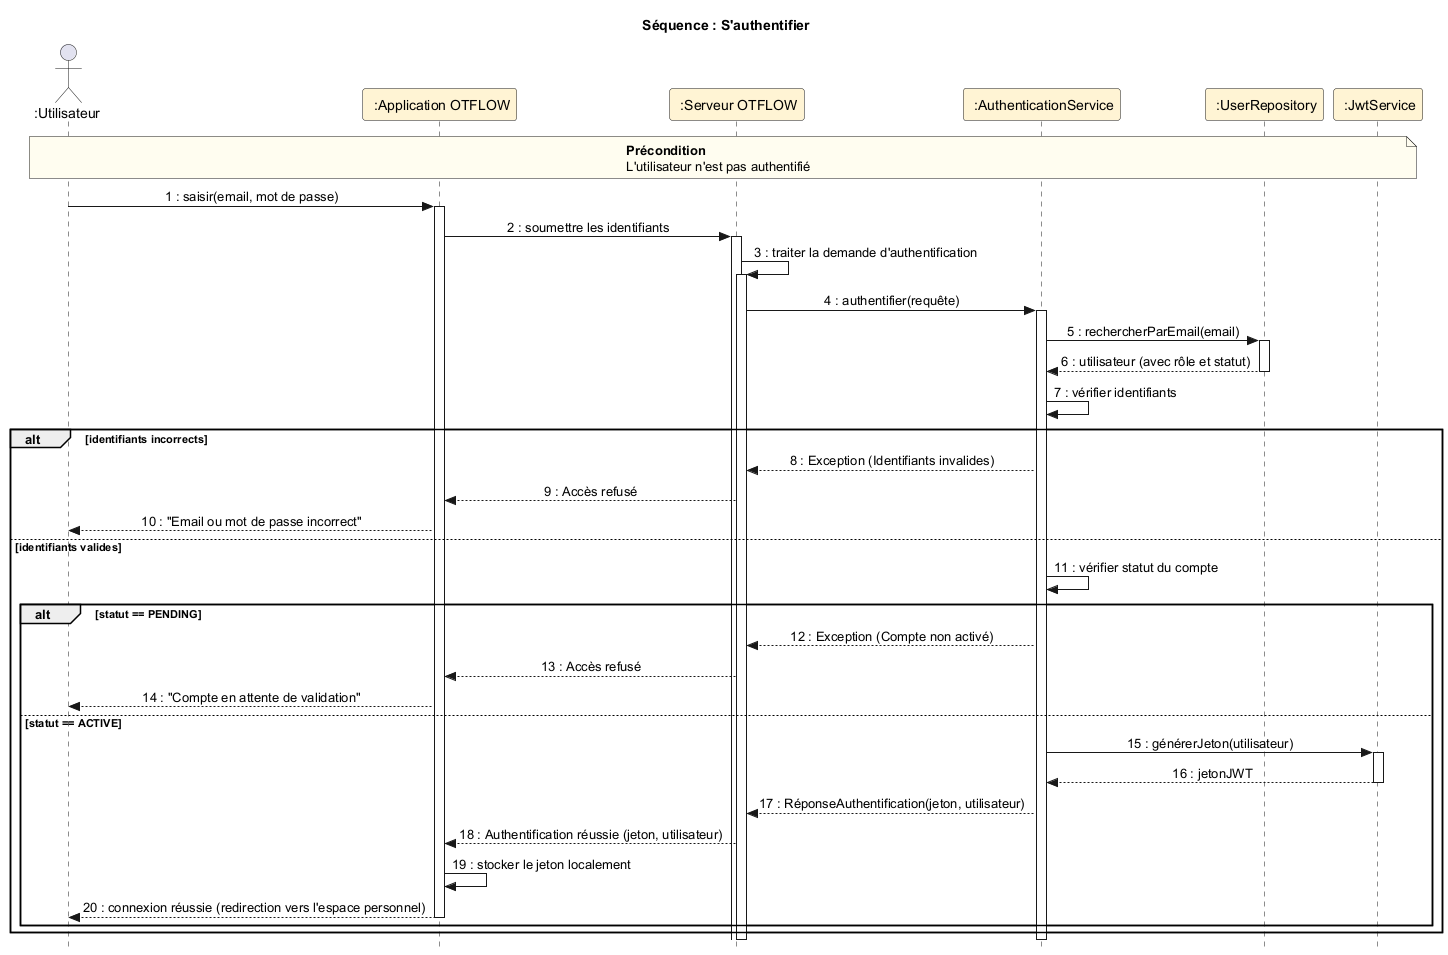
\includegraphics[width=0.85\textwidth, keepaspectratio]{seq_authentifier.png}
\caption{Diagramme de séquence -- Authentification JWT}
\end{figure}

\subsection{Créer un compte et activer}
Le client saisit ses informations sur le formulaire d'inscription. Le backend enregistre le compte en statut \texttt{PENDING}. L'administrateur valide la demande depuis son interface, ce qui active le compte et déclenche l'envoi d'un email de confirmation. L'utilisateur peut alors se connecter.

\begin{figure}[H]
\centering
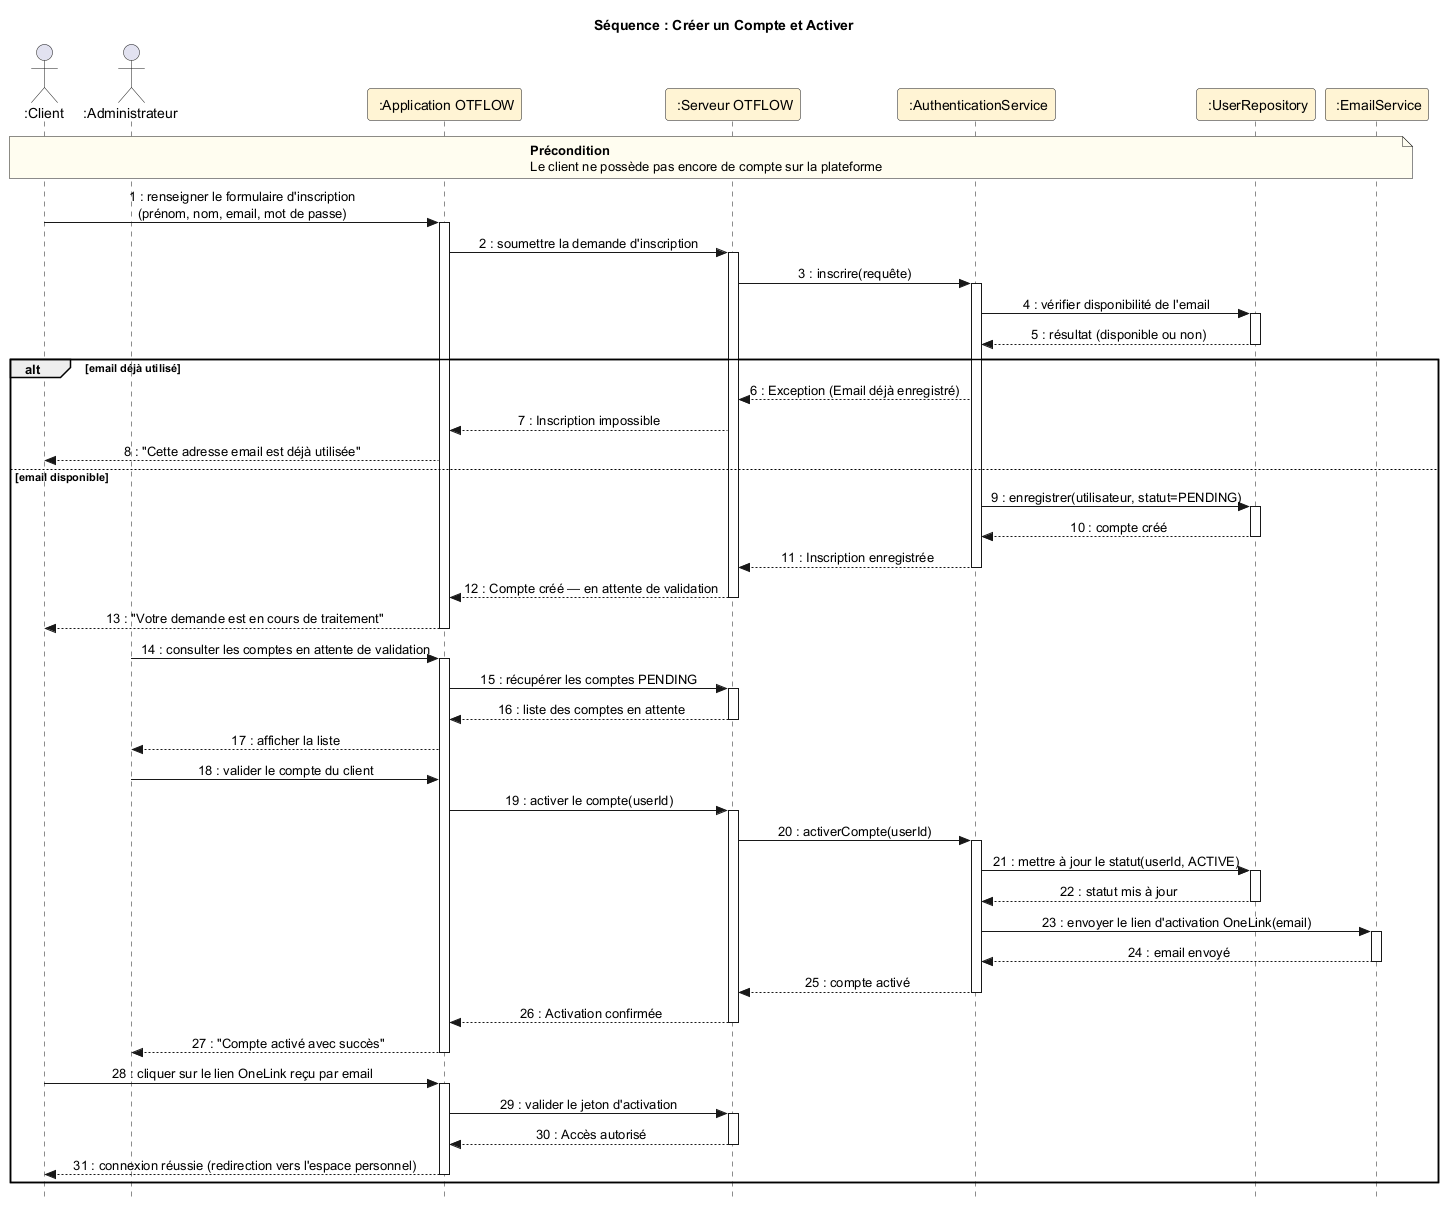
\includegraphics[width=0.85\textwidth, keepaspectratio]{seq_inscription.png}
\caption{Diagramme de séquence -- Inscription et activation du compte}
\end{figure}

\subsection{Réinitialisation du mot de passe}
En cas de perte du mot de passe, l'utilisateur sollicite une réinitialisation. Le backend génère un code sécurisé envoyé par email. L'utilisateur saisit ce code ainsi que son nouveau mot de passe pour valider le changement.

\begin{figure}[H]
\centering
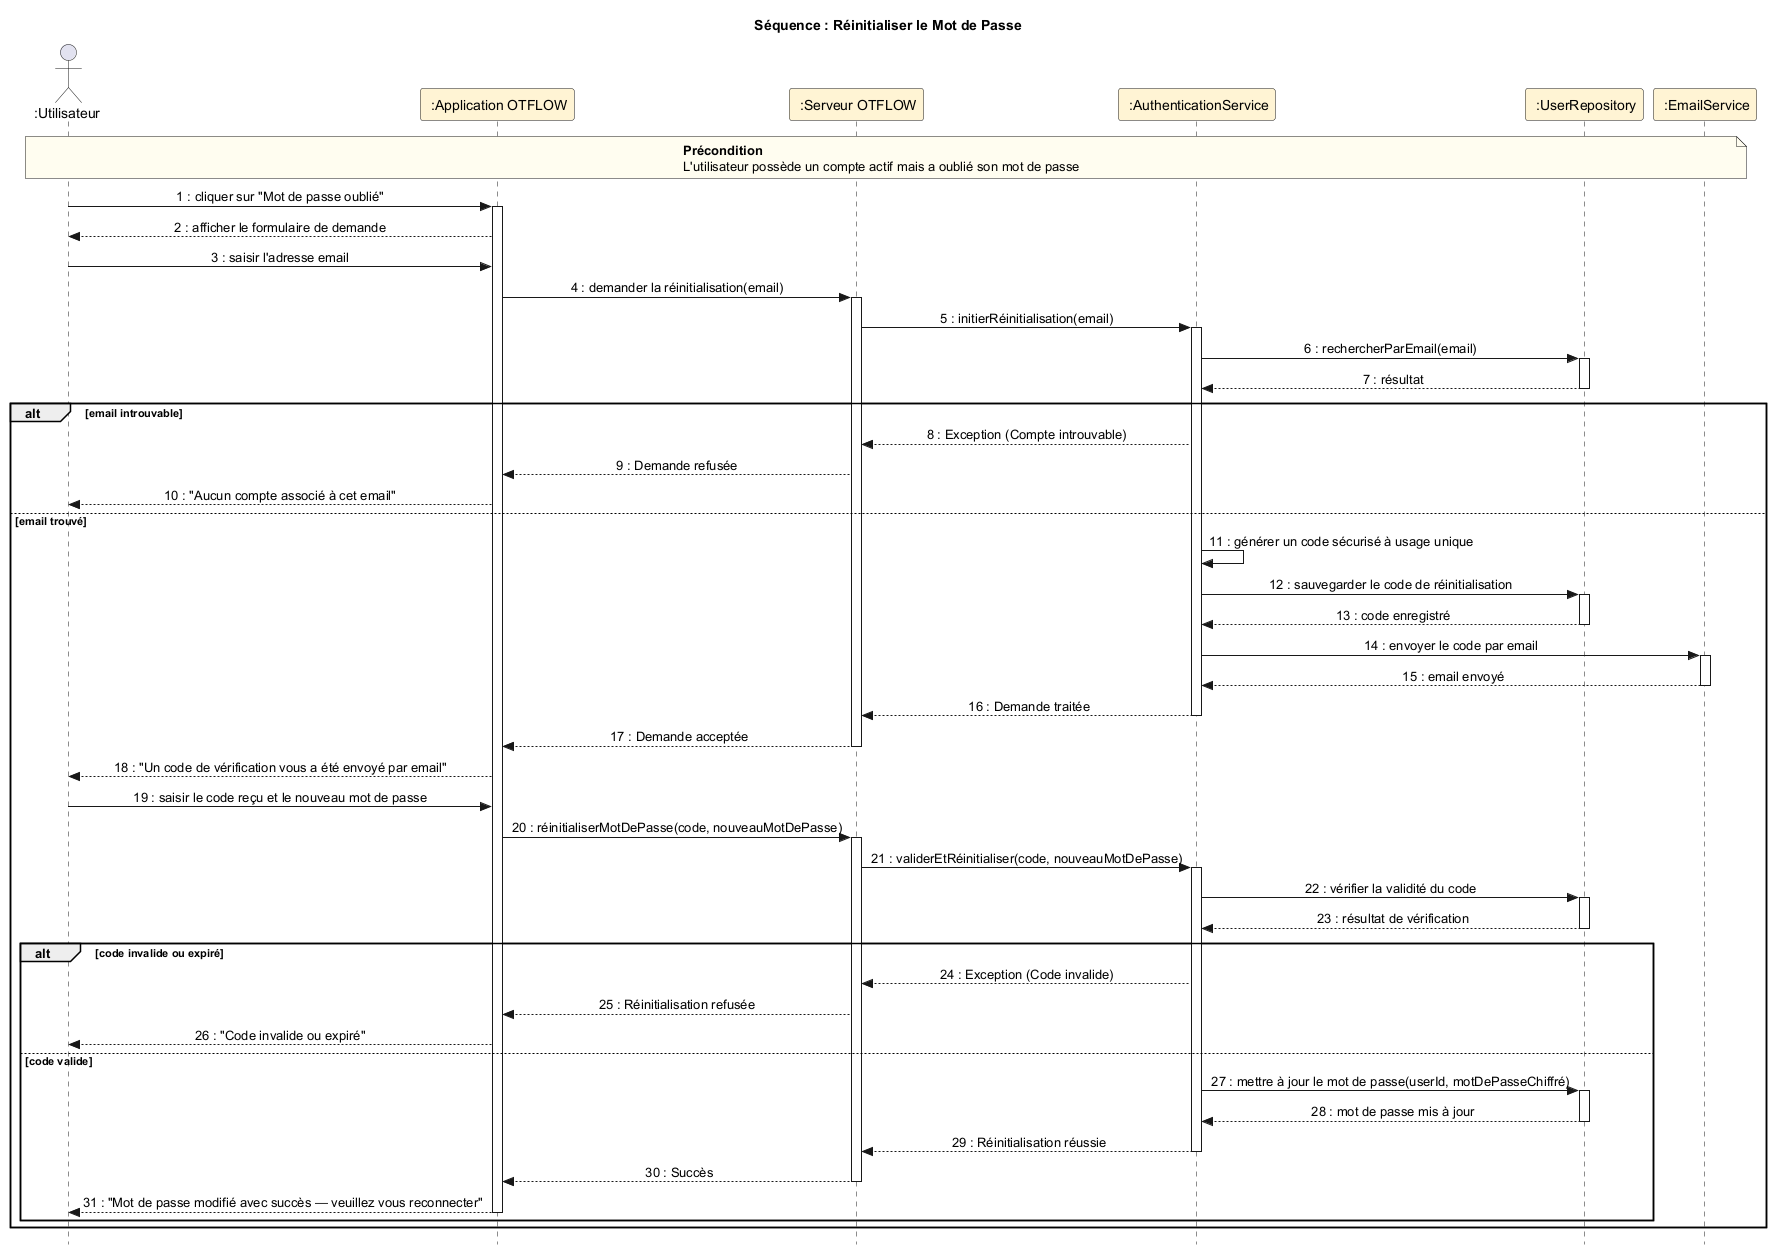
\includegraphics[width=0.85\textwidth, keepaspectratio]{sdresetpassword.png}
\caption{Diagramme de séquence -- Réinitialisation du mot de passe oublié}
\end{figure}

\section{Réalisation}

\subsection{Interface d'inscription}
Le formulaire permet au client de renseigner ses informations (prénom, nom, email, mot de passe). Le compte est créé en statut \texttt{PENDING} en attente de validation administrative.

\begin{figure}[H]
\centering
\includegraphics[width=0.55\linewidth]{inscription.png}
\caption{Interface d'inscription}
\end{figure}

\subsection{Interface de connexion}
La page de connexion authentifie l'utilisateur via email et mot de passe, génère un token JWT et redirige automatiquement vers l'espace personnel selon les permissions.

\begin{figure}[H]
\centering
\includegraphics[width=0.55\linewidth]{connexionpng.png}
\caption{Interface de connexion}
\end{figure}

\section{Conclusion}
Ce sprint a mis en place le socle sécuritaire de la plateforme. L'authentification JWT et le système de permissions granulaires assurent un contrôle strict des accès, préparant le développement des fonctionnalités métier des sprints suivants.

% =================================================
\chapter{Sprint 2 -- Administration et Gestion des Utilisateurs}

\section{Introduction}
Le Sprint 2 développe l'espace d'administration de la plateforme OTFLOW. Il couvre la gestion des utilisateurs, des clients, des articles et des permissions. Ces fonctionnalités constituent le socle organisationnel de l'application, permettant à l'administrateur de contrôler finement les accès et les données de référence avant tout traitement des ordres.

\section{Sprint Backlog}

\begin{table}[H]
\centering
\caption{Sprint Backlog -- Sprint 2}
\begin{tabular}{|c|p{4.2cm}|p{5.2cm}|c|}
\hline
\textbf{ID} & \textbf{User Story} & \textbf{Tâche} & \textbf{Durée} \\
\hline
S2-T1 & Gérer les utilisateurs & CRUD utilisateurs + activation/désactivation & 3 jours \\
\hline
S2-T2 & Gérer les permissions & Attribution granulaire par module et par profil & 2 jours \\
\hline
S2-T3 & Gérer les clients & CRUD clients + recherche + mise à jour auto & 2 jours \\
\hline
S2-T4 & Gérer les articles & CRUD articles + catégorisation & 2 jours \\
\hline
\end{tabular}
\end{table}

\section{Diagramme de cas d'utilisation}

\begin{figure}[H]
\centering
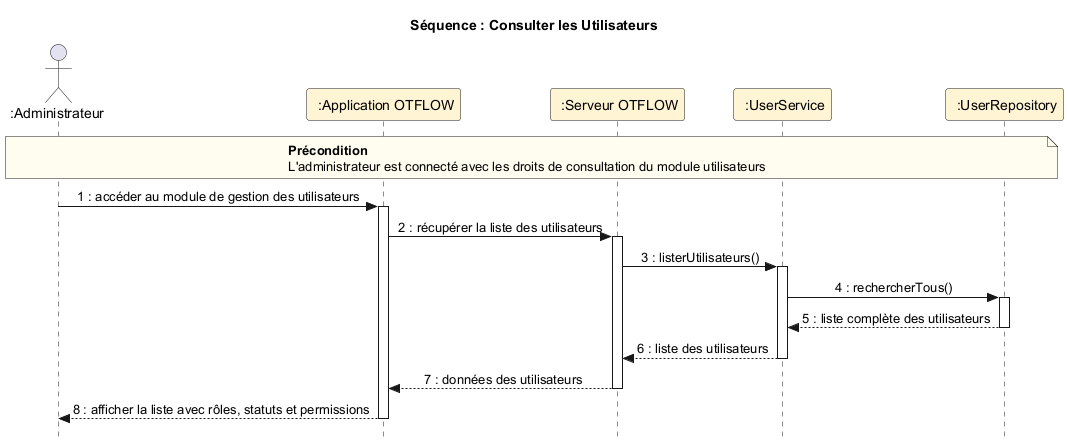
\includegraphics[width=0.85\textwidth, keepaspectratio]{seq_consulter.png}
\caption{Diagramme de séquence -- Consultation des utilisateurs}
\end{figure}

\section{Diagrammes de séquence}

\subsection{Gérer les utilisateurs et les permissions}
L'administrateur accède au module de gestion des utilisateurs. Il peut créer, modifier, activer ou désactiver un compte. Lors de l'attribution des permissions, le système applique les droits sélectionnés au profil de l'utilisateur ; le menu de navigation se reconfigure dynamiquement lors de la prochaine connexion de l'utilisateur concerné.

\begin{figure}[H]
\centering
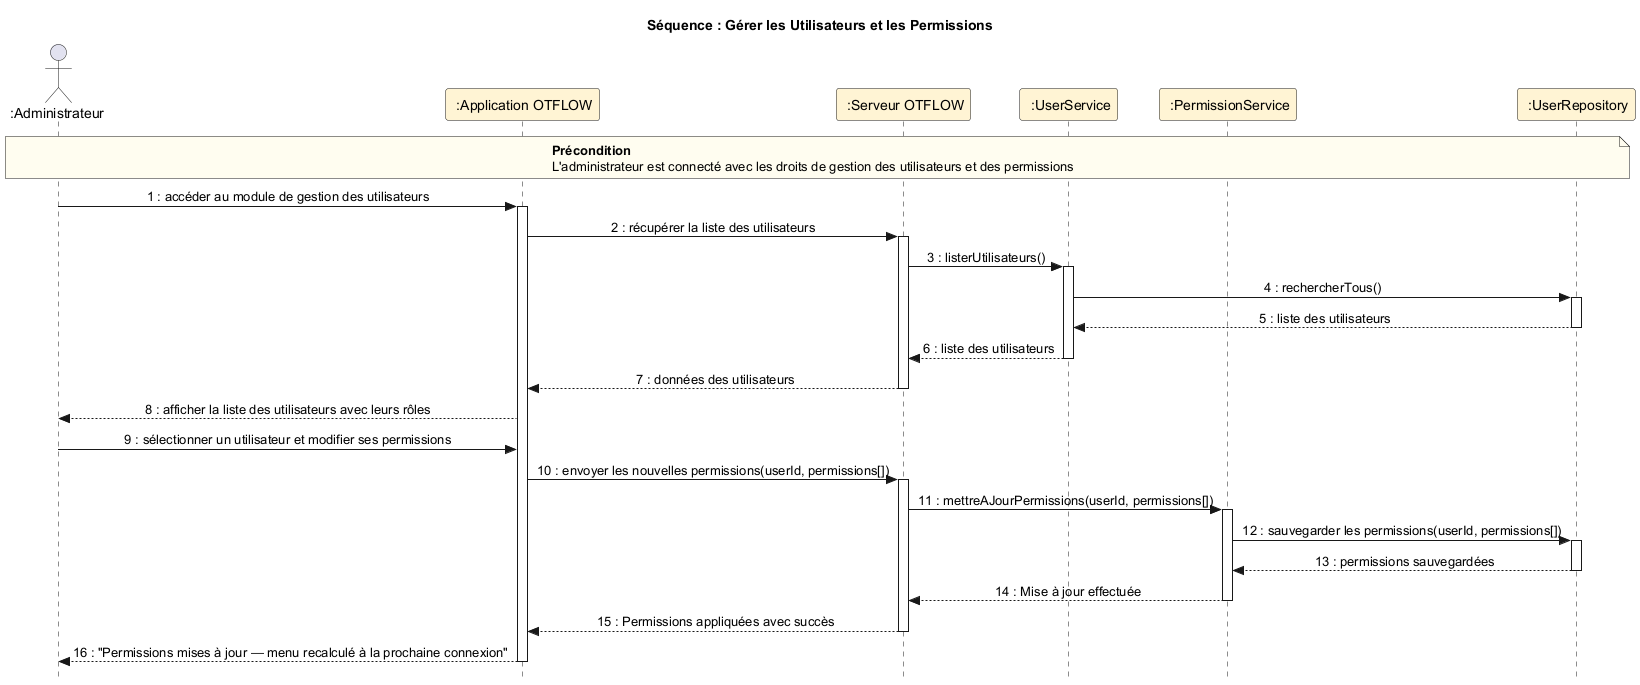
\includegraphics[width=0.85\textwidth, keepaspectratio]{08_ParamPermissions.png}
\caption{Diagramme de séquence -- Gestion des utilisateurs et permissions}
\end{figure}

\subsection{Suppression d'un utilisateur}
L'administrateur peut révoquer l'accès d'un utilisateur en supprimant son compte. Le système vérifie l'absence de dépendances critiques avant de confirmer la suppression définitive en base de données.

\begin{figure}[H]
\centering
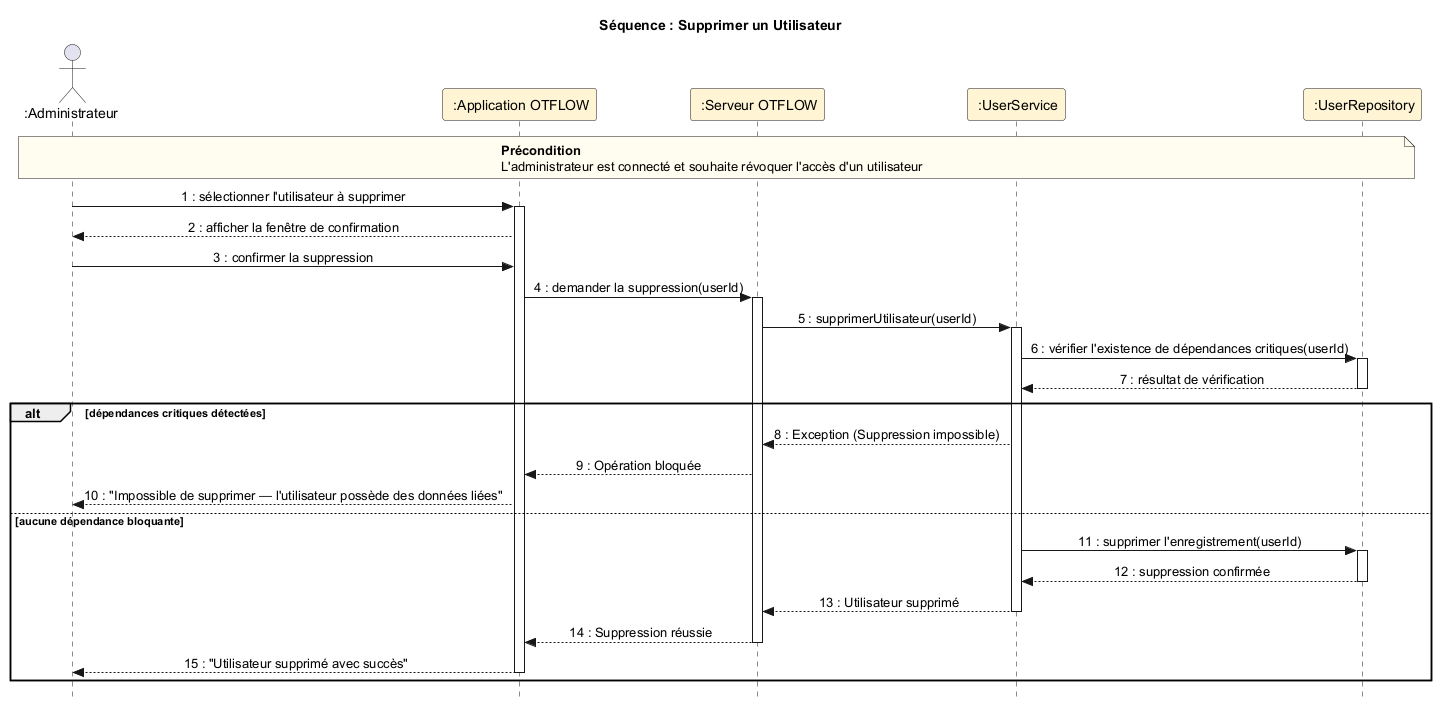
\includegraphics[width=0.85\textwidth, keepaspectratio]{sdsuppression_utilisateur.png}
\caption{Diagramme de séquence -- Suppression d'un utilisateur}
\end{figure}

\subsection{Gérer les clients}
Le commercial ou l'administrateur accède au module clients. Il peut ajouter un nouveau client en renseignant ses coordonnées, son code et son site, ou modifier un client existant. La liste se rafraîchit automatiquement et un module de recherche permet un filtrage rapide par nom ou code client.

\begin{figure}[H]
\centering
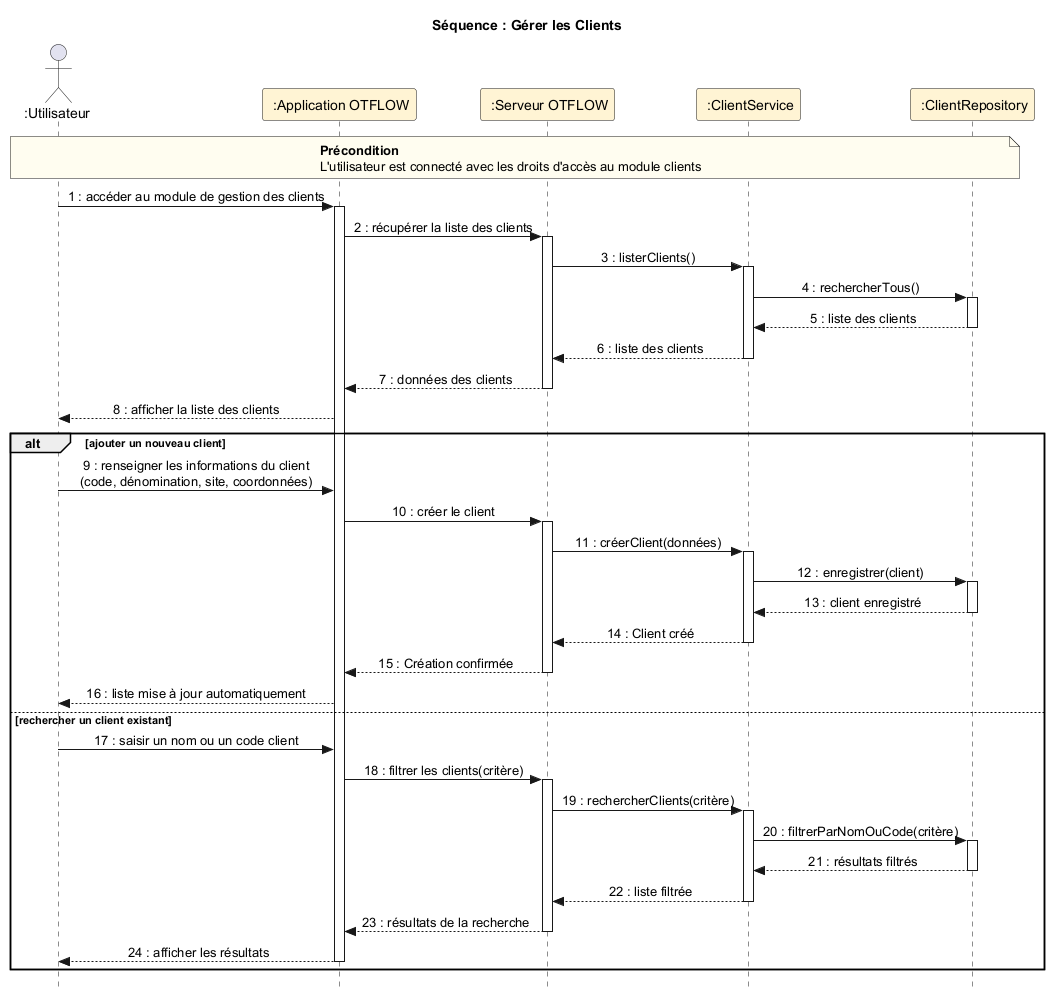
\includegraphics[width=0.85\textwidth, keepaspectratio]{Client01_Consulter.png}
\caption{Diagramme de séquence -- Gestion des clients}
\end{figure}

\subsection{Modification d'un client}
L'utilisateur peut mettre à jour les informations d'un client existant. Le backend valide les modifications et les persiste en base de données.

\begin{figure}[H]
\centering
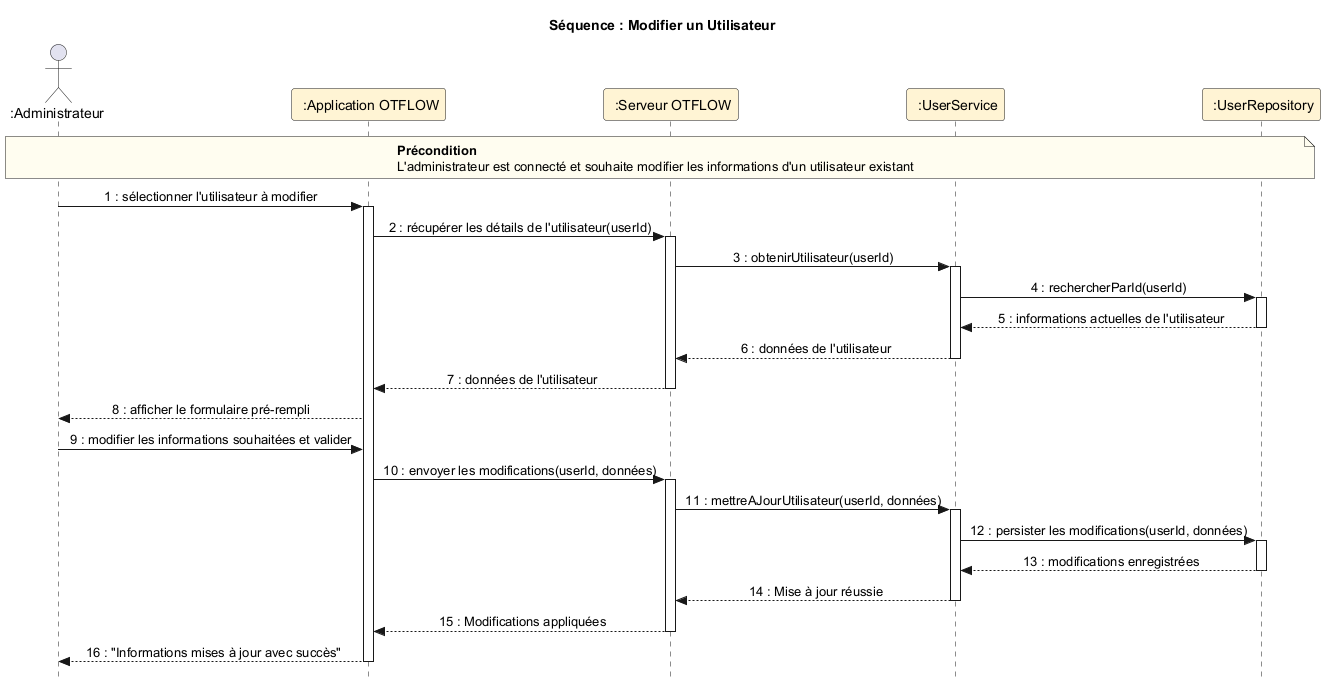
\includegraphics[width=0.85\textwidth, keepaspectratio]{seq_modif_utilisateur.png}
\caption{Diagramme de séquence -- Modification d'un utilisateur}
\end{figure}

\section{Réalisation}

\subsection{Interface de gestion des utilisateurs}
L'administrateur peut consulter la liste complète des comptes, ajouter un utilisateur, modifier ses informations ou activer/désactiver son accès. Chaque compte dispose d'un rôle (Administrateur, Commercial, User-Lumière, Client) et d'un ensemble de permissions configurables par module.

\begin{figure}[H]
\centering
\includegraphics[width=0.75\linewidth]{Pageutilisateur.png}
\caption{Interface de gestion des utilisateurs}
\end{figure}

\begin{figure}[H]
\centering
\includegraphics[width=0.55\linewidth]{AjoutUser.png}
\caption{Fenêtre d'ajout d'un nouvel utilisateur}
\end{figure}

\subsection{Interface de gestion des permissions}
Le module de permissions granulaires permet à l'administrateur d'activer ou de désactiver l'accès à chaque module de l'application (Clients, Articles, Ordres, Dashboard, Utilisateurs) pour chaque profil utilisateur. Le menu de navigation s'adapte dynamiquement en fonction des droits accordés.

\begin{figure}[H]
\centering
\includegraphics[width=0.75\linewidth]{PagePermissionParUSER.png}
\caption{Interface de gestion des permissions par profil}
\end{figure}

\subsection{Interface de gestion des clients}
La liste des clients affiche le code, la dénomination, le site et les coordonnées de chaque client. Elle se met à jour automatiquement. Un module de recherche par nom ou code permet un filtrage rapide.

\begin{figure}[H]
\centering
\includegraphics[width=0.75\linewidth]{PageClient.png}
\caption{Interface de gestion des clients}
\end{figure}

\begin{figure}[H]
\centering
\includegraphics[width=0.55\linewidth]{AjoutClient.png}
\caption{Fenêtre de création d'un client}
\end{figure}

\begin{figure}[H]
\centering
\includegraphics[width=0.75\linewidth]{PageClientOnAttends.png}
\caption{Interface des clients en attente de validation}
\end{figure}

\subsection{Interface de gestion des articles}
Le module articles permet de référencer les produits transportés. Chaque article est défini par un code, une désignation, une unité de mesure et une catégorie. L'administrateur peut ajouter, modifier ou archiver un article depuis cette interface.

\begin{figure}[H]
\centering
\includegraphics[width=0.75\linewidth]{PageArticle.png}
\caption{Interface de gestion des articles}
\end{figure}

\begin{figure}[H]
\centering
\includegraphics[width=0.55\linewidth]{AjoutArticle.png}
\caption{Fenêtre d'ajout d'un article}
\end{figure}

\section{Conclusion}
Ce sprint a livré l'ensemble des fonctionnalités d'administration : gestion fine des utilisateurs, attribution de permissions granulaires par module, gestion des clients et référencement des articles. Ces éléments constituent la base de données de référence sur laquelle repose la gestion des ordres développée au sprint suivant.

% =================================================
\chapter{Sprint 3 -- Gestion des Ordres et Suivi Cartographique}

\section{Introduction}
Le Sprint 3 couvre le cœur opérationnel de la plateforme : la création des ordres de transport, leur confirmation, leur suivi avec génération automatique du fichier PLA, ainsi que le module cartographique permettant le live tracking et le replay des trajets via Leaflet et OpenStreetMap.

\section{Sprint Backlog}

\begin{table}[H]
\centering
\caption{Sprint Backlog -- Sprint 3}
\begin{tabular}{|c|p{4.2cm}|p{5.2cm}|c|}
\hline
\textbf{ID} & \textbf{User Story} & \textbf{Tâche} & \textbf{Durée} \\
\hline
S3-T1 & Créer un ordre de transport & Formulaire de saisie multi-champs & 2 jours \\
\hline
S3-T2 & Confirmer un ordre et générer le fichier PLA & Validation + génération automatique PLA & 2 jours \\
\hline
S3-T3 & Suivre les ordres avec confidentialité & Liste filtrée par profil + auto-refresh & 2 jours \\
\hline
S3-T4 & Voir la position du camion en temps réel & Intégration Leaflet + API GPS Rimtrack & 3 jours \\
\hline
S3-T5 & Rejouer le trajet après livraison & Algorithme replay + polyline GPS & 2 jours \\
\hline
S3-T6 & Voir la progression des étapes & Timeline alimentée par Mobilité Lumière & 2 jours \\
\hline
S3-T7 & Réconcilier matricule TMS et boîtier GPS & Algorithme Flexible Plate Matching & 1 jour \\
\hline
\end{tabular}
\end{table}

\section{Diagramme de cas d'utilisation}

\begin{figure}[H]
\centering
\fbox{\parbox{0.85\textwidth}{\centering
\vspace{3.5cm}
\textit{[Insérer ici le diagramme de cas d'utilisation -- Sprint 3]}
\vspace{3.5cm}
}}
\caption{Diagramme de cas d'utilisation -- Sprint 3}
\end{figure}

\section{Diagrammes de séquence}

\subsection{Créer un ordre de transport}
Le commercial remplit le formulaire de création. Le frontend envoie les données au backend via une requête POST sécurisée. Le backend valide, persiste l'ordre en base avec le statut \texttt{EN\_ATTENTE} et retourne une confirmation. L'ordre apparaît dans la liste des ordres non confirmés.

\begin{figure}[H]
\centering
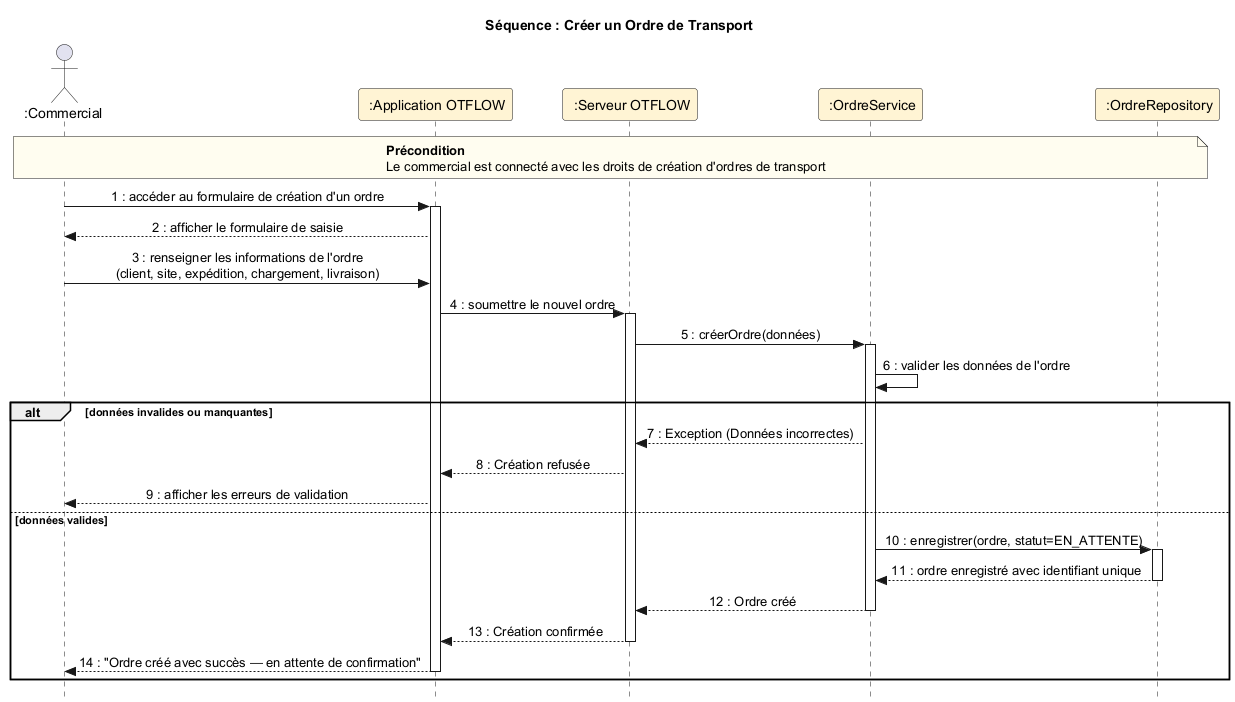
\includegraphics[width=0.85\textwidth, keepaspectratio]{sdnouvelordre.png}
\caption{Diagramme de séquence -- Création d'un ordre de transport}
\end{figure}

\subsection{Confirmer un ordre et générer le fichier PLA}
Lorsque le commercial valide un ordre, le backend fait passer son statut à \texttt{CONFIRMÉ} et déclenche automatiquement la génération du fichier PLA correspondant. Ce fichier est immédiatement transmis au TMS externe pour planification.

\begin{figure}[H]
\centering
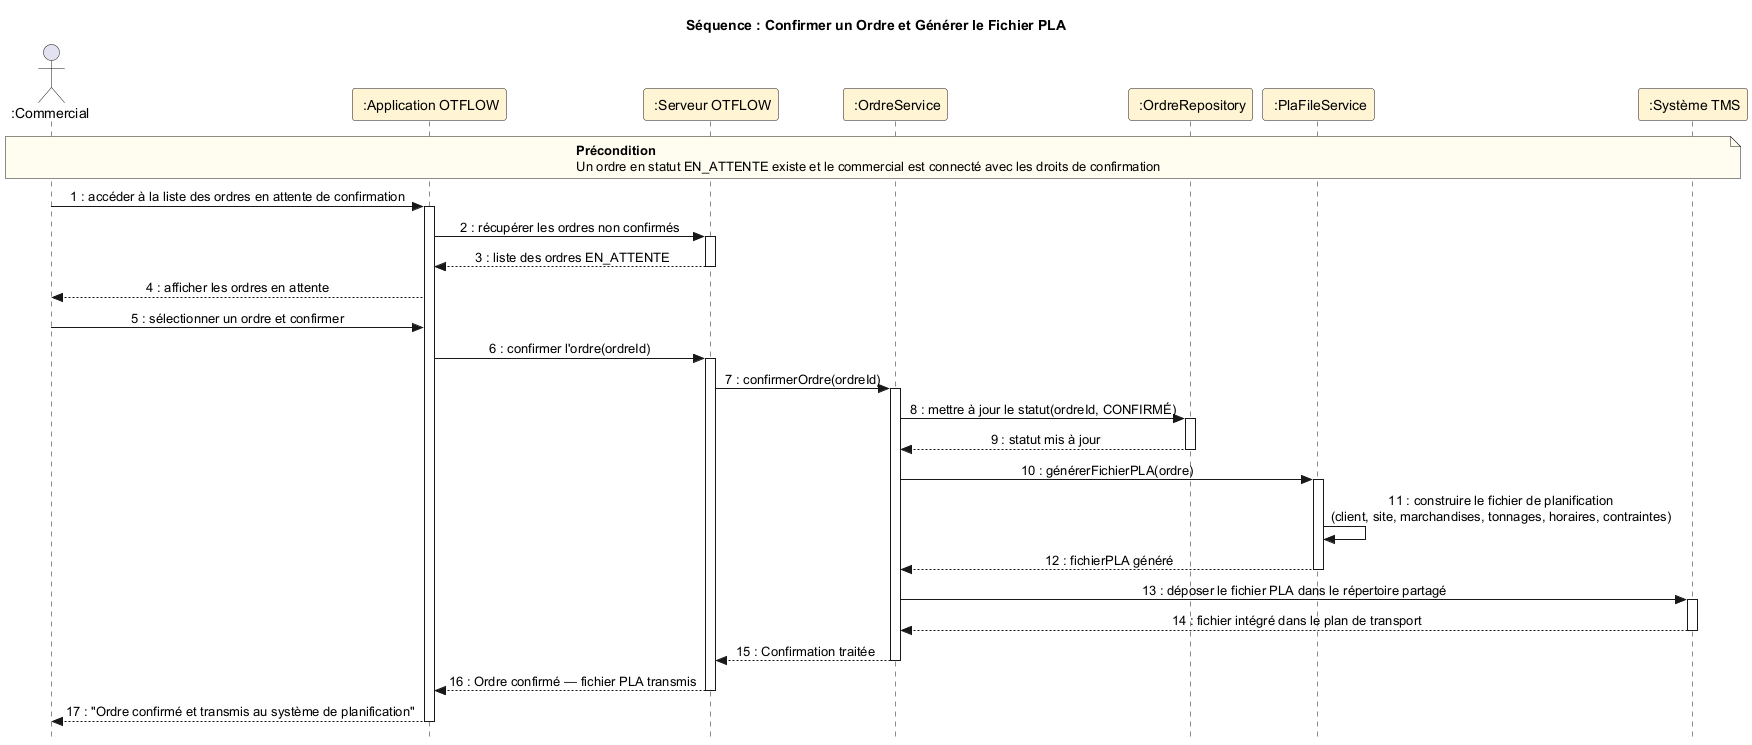
\includegraphics[width=0.85\textwidth, keepaspectratio]{sd_confirmation_pla.png}
\caption{Diagramme de séquence -- Confirmation d'un ordre et génération du fichier PLA}
\end{figure}

\subsection{Consulter les ordres avec isolation des données}
Lors de l'accès à la liste des ordres, le backend applique un filtre basé sur le profil connecté : un client ne voit que ses propres ordres du jour, tandis que les commerciaux et administrateurs ont une vue complète.

\begin{figure}[H]
\centering
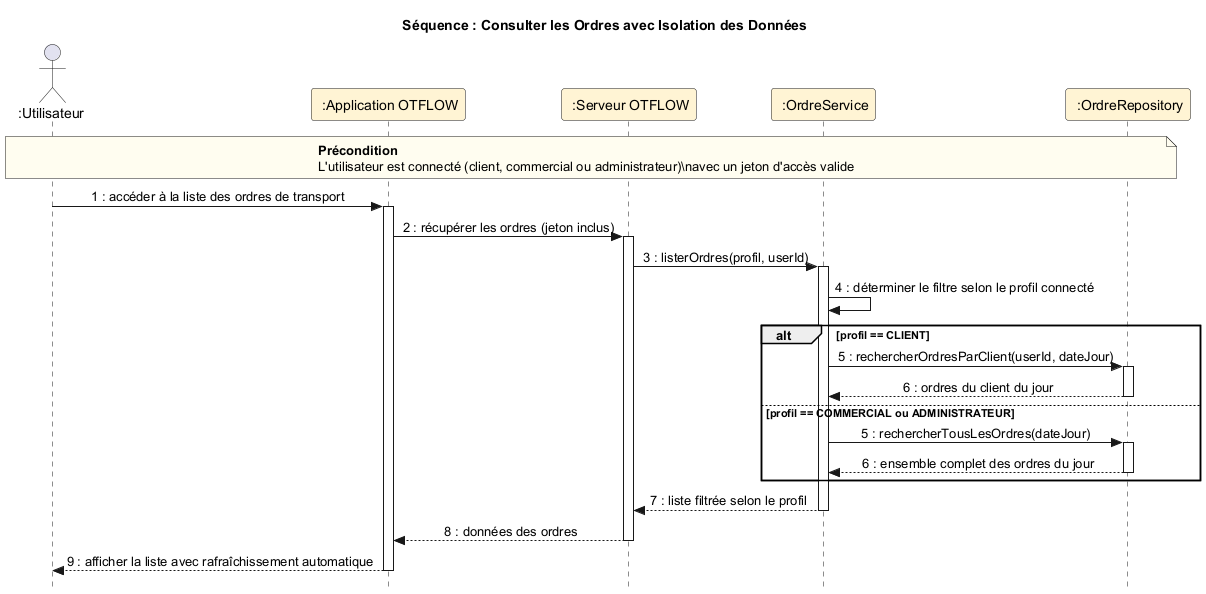
\includegraphics[width=0.85\textwidth, keepaspectratio]{sdsuivi_et_tracking.png}
\caption{Diagramme de séquence -- Consultation des ordres avec confidentialité}
\end{figure}

\subsection{Live Tracking GPS}
L'utilisateur sélectionne un ordre actif. Le frontend interroge le backend, qui récupère les coordonnées GPS en temps réel depuis Rimtrack via l'algorithme de réconciliation. Les coordonnées sont retournées et affichées sur la carte Leaflet avec un marqueur animé indiquant la position du camion.

\begin{figure}[H]
\centering
\includegraphics[width=0.85\textwidth, keepaspectratio]{06_LiveTrackingGPS.png}
\caption{Diagramme de séquence -- Live Tracking GPS}
\end{figure}

\section{Réalisation}

\subsection{Création des ordres}
Le formulaire de création collecte les informations du client, le site d'exploitation, les détails de l'expédition et les informations de chargement et de livraison. L'ordre est enregistré en statut \texttt{EN\_ATTENTE} jusqu'à sa confirmation par le commercial.

\begin{figure}[H]
\centering
\includegraphics[width=0.75\linewidth]{CreeOrdre.png}
\caption{Interface de création d'un ordre -- Étape 1}
\end{figure}

\begin{figure}[H]
\centering
\includegraphics[width=0.75\linewidth]{CreeOrdre2.png}
\caption{Interface de création d'un ordre -- Étape 2}
\end{figure}

\subsection{Confirmation des ordres et génération du fichier PLA}

\subsubsection{Qu'est-ce que le fichier PLA ?}
Le fichier \textbf{PLA} (fichier de PLAnification) est un fichier structuré généré automatiquement par OTFLOW au moment de la confirmation d'un ordre de transport. Il constitue l'interface de communication entre OTFLOW et le TMS externe de Lumière Transports.

Ce fichier contient l'ensemble des informations nécessaires à la planification de la tournée : le numéro de l'ordre, le client, le site d'enlèvement, l'adresse de livraison, la nature des marchandises, les tonnages, les horaires prévus et les contraintes particulières. Une fois généré, le fichier PLA est déposé dans un répertoire partagé lu par le TMS, qui l'intègre automatiquement dans son plan de transport.

Cette génération automatique élimine toute ressaisie manuelle des données et garantit la cohérence de l'information entre les deux systèmes.

\begin{figure}[H]
\centering
\includegraphics[width=0.75\linewidth]{PageOrdreNonConfirme.png}
\caption{Interface des ordres en attente de confirmation}
\end{figure}

\begin{figure}[H]
\centering
\includegraphics[width=0.75\linewidth]{Planification.png}
\caption{Exemple de fichier PLA généré automatiquement après confirmation}
\end{figure}

\subsection{Suivi des ordres}
La liste de suivi affiche les ordres du jour par défaut, filtrés selon le profil connecté. Elle se met à jour automatiquement. Un module de recherche par nom ou code permet un filtrage rapide.

\begin{figure}[H]
\centering
\includegraphics[width=0.75\linewidth]{SuiviOrdre.png}
\caption{Interface de suivi des ordres avec filtres et auto-refresh}
\end{figure}

\subsection{Timeline de progression et cartographie}
Chaque ordre confirmé affiche une timeline graphique des événements logistiques (Départ, Chargement, Transport, Livraison, Validation) alimentée par les statuts de Mobilité Lumière. La carte Leaflet/OpenStreetMap intégrée permet de visualiser le trajet en temps réel ou en replay historique, avec calcul de la distance réelle et tooltips de vitesse sur chaque point.

\begin{figure}[H]
\centering
\includegraphics[width=0.75\linewidth]{DetailOrdre.png}
\caption{Progression d'un ordre : timeline et visualisation cartographique}
\end{figure}

\begin{figure}[H]
\centering
\includegraphics[width=0.75\linewidth]{DetailSuivi.png}
\caption{Détail du suivi cartographique -- Live tracking et replay GPS}
\end{figure}

\section{Conclusion}
Ce sprint a livré le cœur opérationnel de la plateforme : création et confirmation des ordres avec génération automatique du fichier PLA vers le TMS, suivi filtré par profil utilisateur, et module cartographique complet intégrant live tracking et replay historique GPS.

% =================================================
\chapter{Sprint 4 -- Application Mobile Client}

\section{Introduction}
Le Sprint 4 développe l'application mobile \textbf{OTFLOW} destinée aux clients. Construite avec Ionic et Angular, déployée sur Android via Capacitor, elle regroupe l'ensemble des fonctionnalités client : authentification sécurisée, gestion des commandes, suivi cartographique, notifications et gestion des rappels.

\section{Sprint Backlog}

\begin{table}[H]
\centering
\caption{Sprint Backlog -- Sprint 4}
\begin{tabular}{|c|p{4.2cm}|p{5.2cm}|c|}
\hline
\textbf{ID} & \textbf{User Story} & \textbf{Tâche} & \textbf{Durée} \\
\hline
S4-T1 & Mettre en place l'architecture mobile & Ionic + Capacitor + Routes & 2 jours \\
\hline
S4-T2 & S'authentifier sur mobile & Login + JWT + OneLink & 2 jours \\
\hline
S4-T3 & Accéder à un tableau de bord & Page Home + actions rapides + brouillons & 2 jours \\
\hline
S4-T4 & Gérer mes rappels & CRUD rappels groupés par date & 2 jours \\
\hline
S4-T5 & Créer et consulter mes ordres & Formulaire + liste + détail & 3 jours \\
\hline
S4-T6 & Suivre mes livraisons & Stepper + tracking temps réel & 3 jours \\
\hline
S4-T7 & Visualiser la carte & Leaflet/OSM + permissions GPS Android & 2 jours \\
\hline
S4-T8 & Recevoir des notifications & Notifications push + email & 2 jours \\
\hline
\end{tabular}
\end{table}

\section{Diagramme de cas d'utilisation}

\begin{figure}[H]
\centering
\includegraphics[width=0.85\textwidth, keepaspectratio]{uc_mobile.png}
\caption{Diagramme de cas d'utilisation -- Application mobile client}
\end{figure}

\section{Diagrammes de séquence}

\subsection{Connexion et Sécurisation (Mobile)}
Le client saisit ses identifiants. L'application interroge le backend qui retourne un token JWT. Ce token est persisté de manière sécurisée dans le stockage local natif via Capacitor Preferences, garantissant le maintien de la session.

\begin{figure}[H]
\centering
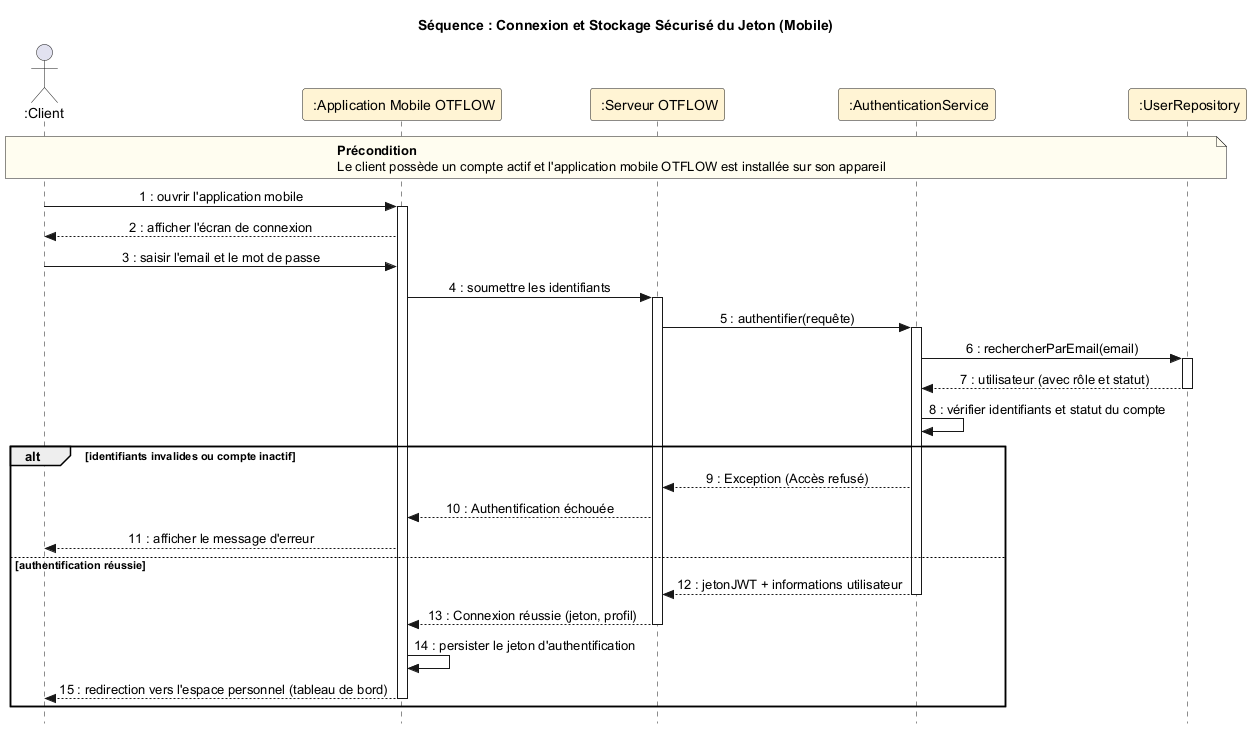
\includegraphics[width=0.85\textwidth, keepaspectratio]{sd_login_mobile.png}
\caption{Diagramme de séquence -- Connexion et Stockage Local (Mobile)}
\end{figure}

\subsection{Notification Push et Temps Réel (Mobile)}
Lors d'un changement de statut par le chauffeur, le backend notifie le client via Firebase Cloud Messaging (FCM). L'application mobile intercepte la notification, génère un retour haptique (vibration) et actualise instantanément le stepper de livraison.

\begin{figure}[H]
\centering
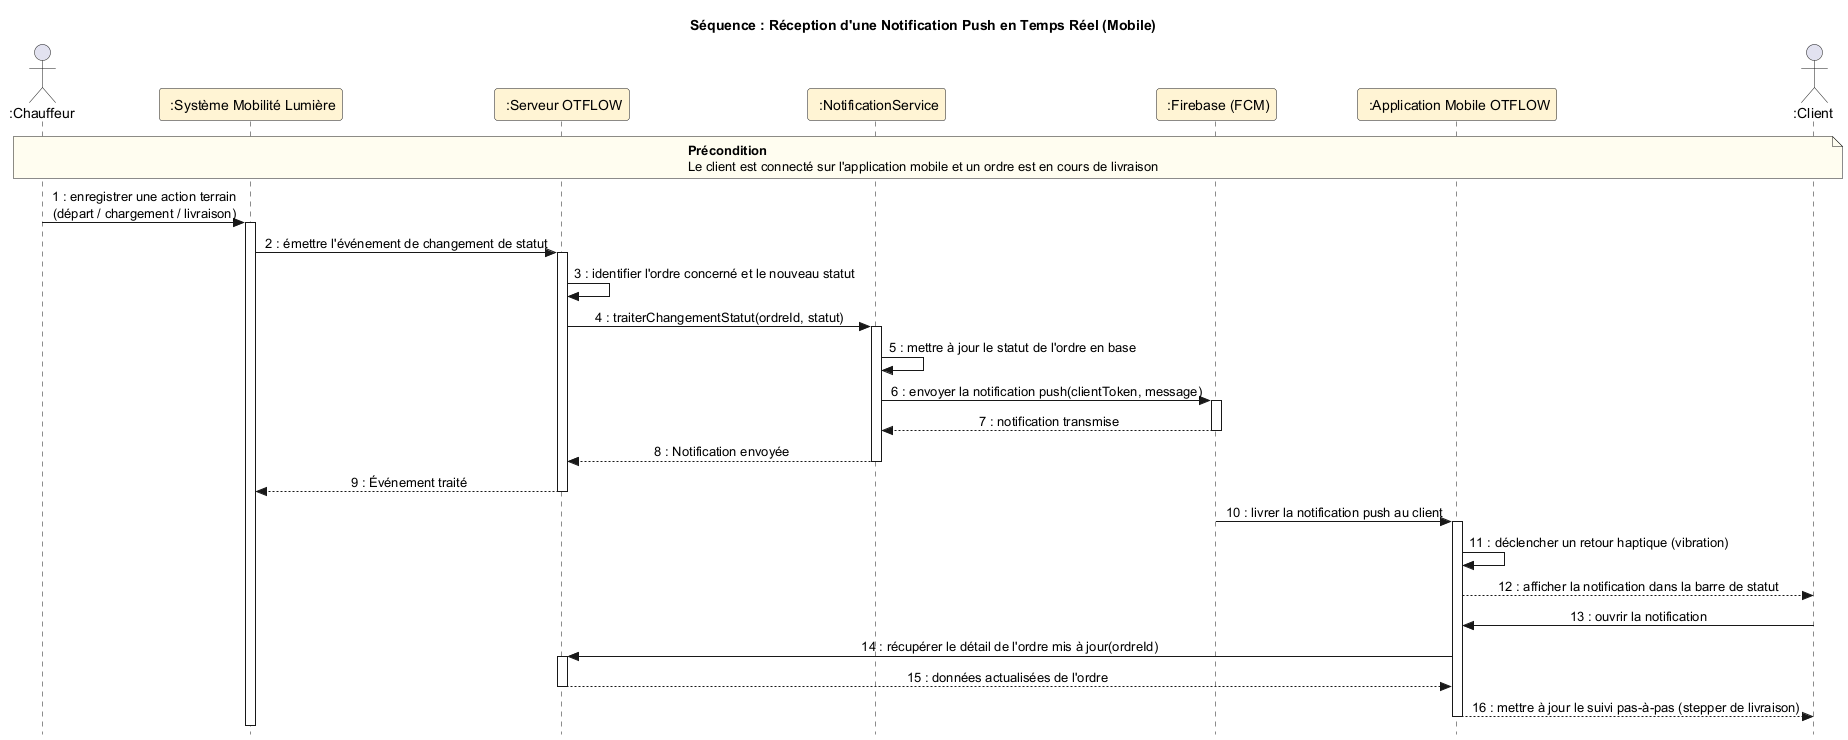
\includegraphics[width=0.85\textwidth, keepaspectratio]{sd_push_mobile.png}
\caption{Diagramme de séquence -- Réception d'une Notification Push (Temps Réel)}
\end{figure}

\section{Réalisation}

\subsection{Authentification et inscription}

\begin{figure}[H]
\centering
\begin{minipage}{0.3\textwidth}
\centering
\includegraphics[width=3.5cm, height=7cm, keepaspectratio]{page_register_mobile.png}
\caption{Formulaire d'inscription}
\end{minipage}
\hfill
\begin{minipage}{0.3\textwidth}
\centering
\includegraphics[width=3.5cm, height=7cm, keepaspectratio]{mobile_pending.png}
\caption{Page d'attente (PENDING)}
\end{minipage}
\hfill
\begin{minipage}{0.3\textwidth}
\centering
\includegraphics[width=3.5cm, height=7cm, keepaspectratio]{page_login_mobile.png}
\caption{Interface de connexion}
\end{minipage}

\vspace{0.3cm}

\includegraphics[width=8cm, keepaspectratio]{mobile_email_activation.png}
\caption{Email d'activation avec lien OneLink}
\end{figure}

\subsection{Tableau de bord et rappels}
Le tableau de bord de l'application mobile offre aux clients un accès simplifié aux différentes fonctionnalités de la plateforme (création de commandes, suivi cartographique en temps réel, messagerie avec le chatbot). Le module de gestion des rappels permet de configurer des alertes sur l'avancement des livraisons.

\begin{figure}[H]
\centering
\begin{minipage}{0.3\textwidth}
\centering
\includegraphics[width=3.5cm, height=7cm, keepaspectratio]{page_acceuil_mobile.png}
\caption{Tableau de bord}
\end{minipage}
\hfill
\begin{minipage}{0.3\textwidth}
\centering
\includegraphics[width=3.5cm, height=7cm, keepaspectratio]{page_acceuil_fab.png}
\caption{Menu d'actions rapides (FAB)}
\end{minipage}
\hfill
\begin{minipage}{0.3\textwidth}
\centering
\includegraphics[width=3.5cm, height=7cm, keepaspectratio]{mobile_rappels_page.png}
\caption{Création d'un rappel}
\end{minipage}
\end{figure}

Les rappels peuvent être saisis manuellement via un formulaire ou être générés intelligemment par le chatbot IA (Llama 3) à partir des messages échangés. L'utilisateur accède ensuite à la liste des rappels créés et peut cliquer sur l'un d'eux pour en consulter la fiche détaillée.

\begin{figure}[H]
\centering
\begin{minipage}{0.45\textwidth}
\centering
\includegraphics[width=4cm, height=7cm, keepaspectratio]{mobile_rappels_ia.png}
\caption{Liste des rappels générés par l'IA}
\end{minipage}
\hfill
\begin{minipage}{0.45\textwidth}
\centering
\includegraphics[width=4cm, height=7cm, keepaspectratio]{mobile_rappels_details.png}
\caption{Détails et options d'un rappel}
\end{minipage}
\end{figure}

\subsection{Gestion des ordres}

\begin{figure}[H]
\centering
\begin{minipage}{0.3\textwidth}
\centering
\includegraphics[width=3.5cm, height=7cm, keepaspectratio]{nouveau_ordre_mobile.png}
\caption{Nouvelle commande}
\end{minipage}
\hfill
\begin{minipage}{0.3\textwidth}
\centering
\includegraphics[width=3.5cm, height=7cm, keepaspectratio]{page_ordre_mobile.png}
\caption{Mes Ordres}
\end{minipage}
\hfill
\begin{minipage}{0.3\textwidth}
\centering
\includegraphics[width=3.5cm, height=7cm, keepaspectratio]{page_detail_ordre.png}
\caption{Détails d'une commande}
\end{minipage}
\end{figure}

\subsection{Suivi des livraisons et cartographie}

\begin{figure}[H]
\centering
\begin{minipage}{0.3\textwidth}
\centering
\includegraphics[width=3.5cm, height=7cm, keepaspectratio]{page_livraisons_mobile.png}
\caption{Mes livraisons}
\end{minipage}
\hfill
\begin{minipage}{0.3\textwidth}
\centering
\includegraphics[width=3.5cm, height=7cm, keepaspectratio]{page_encoursdelivraison_mobile.png}
\caption{Stepper de livraison}
\end{minipage}
\hfill
\begin{minipage}{0.3\textwidth}
\centering
\includegraphics[width=3.5cm, height=7cm, keepaspectratio]{gps_tracking_mobile.png}
\caption{Tracking temps réel}
\end{minipage}
\end{figure}

\begin{figure}[H]
\centering
\includegraphics[width=4.5cm, height=8cm, keepaspectratio]{page_profile_mobile.png}
\caption{Paramètres et Profil}
\end{figure}

\subsection{Répertoire clients et notifications}

\begin{figure}[H]
\centering
\begin{minipage}{0.45\textwidth}
\centering
\includegraphics[width=4cm, height=7cm, keepaspectratio]{page_client_mobile.png}
\caption{Répertoire clients}
\end{minipage}
\hfill
\begin{minipage}{0.45\textwidth}
\centering
\includegraphics[width=4cm, height=7cm, keepaspectratio]{page_notifications_mobile.png}
\caption{Centre de notifications}
\end{minipage}
\end{figure}

\begin{figure}[H]
\centering
\includegraphics[width=8cm, keepaspectratio]{notif.png}
\caption{Email de notification automatique lors d'un changement de statut}
\end{figure}

\section{Tests}

\begin{table}[H]
\centering
\caption{Résultats des tests -- Sprint 4}
\begin{tabular}{|p{8.5cm}|c|}
\hline
\textbf{Fonctionnalité testée} & \textbf{Résultat} \\
\hline
Inscription et statut PENDING & Validé \\
\hline
Activation via OneLink & Validé \\
\hline
Connexion JWT et protection des routes & Validé \\
\hline
Création d'une commande & Validé \\
\hline
Filtrage et recherche des ordres & Validé \\
\hline
Stepper de progression des livraisons & Validé \\
\hline
Tracking Leaflet et GPS Rimtrack & Validé \\
\hline
Notifications temps réel (push + email) & Validé \\
\hline
\end{tabular}
\end{table}

\section{Conclusion}
Le Sprint 4 livre une application mobile complète et autonome. Le flux OneLink sécurise les inscriptions, le tracking temps réel et le stepper offrent une visibilité totale sur les livraisons, et les notifications push assurent une communication proactive avec le client.

% =================================================
\chapter{Sprint 5 -- Chatbot IA et Outils d'Analyse}

\section{Introduction}
Le Sprint 5 enrichit la plateforme avec deux fonctionnalités avancées : l'assistant intelligent propulsé par le modèle Llama 3 via l'API Groq, disponible sur web et mobile, et des outils d'analyse permettant une supervision synthétique de l'activité logistique.

\section{Sprint Backlog}

\begin{table}[H]
\centering
\caption{Sprint Backlog -- Sprint 5}
\begin{tabular}{|c|p{4.2cm}|p{5.2cm}|c|}
\hline
\textbf{ID} & \textbf{User Story} & \textbf{Tâche} & \textbf{Durée} \\
\hline
S5-T1 & Interagir avec un assistant IA & Interface chatbot + intégration API Groq & 4 jours \\
\hline
S5-T2 & Consulter mes ordres via le chatbot & Connexion chatbot aux données utilisateur & 2 jours \\
\hline
S5-T3 & Visualiser des indicateurs d'activité & Tableau de bord stats + graphiques & 3 jours \\
\hline
S5-T4 & Accéder au chatbot depuis le mobile & Interface chatbot Ionic + API Groq & 3 jours \\
\hline
\end{tabular}
\end{table}

\section{Diagramme de cas d'utilisation}

\begin{figure}[H]
\centering
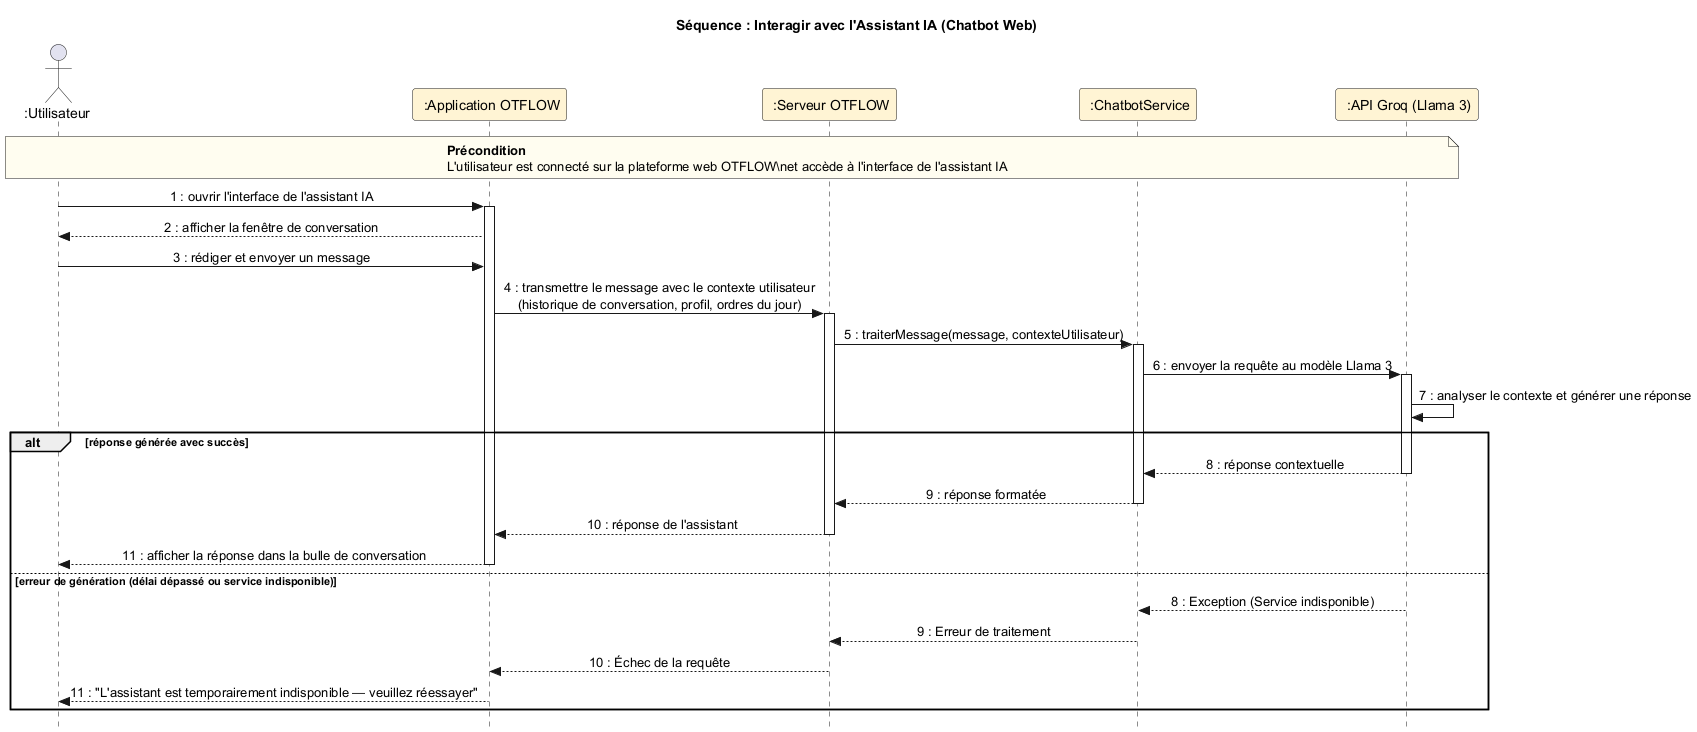
\includegraphics[width=0.85\textwidth, keepaspectratio]{sd_chatbot.png}
\caption{Diagramme de cas d'utilisation -- Sprint 5}
\end{figure}

\section{Diagrammes de séquence}

\subsection{Interaction avec le Chatbot IA}
L'utilisateur envoie un message depuis l'interface web ou mobile. Le frontend transmet la requête au backend, qui la relaie à l'API Groq avec le contexte utilisateur. Le modèle Llama 3 génère une réponse contextuelle retournée au frontend et affichée dans la bulle de conversation.

\begin{figure}[H]
\centering
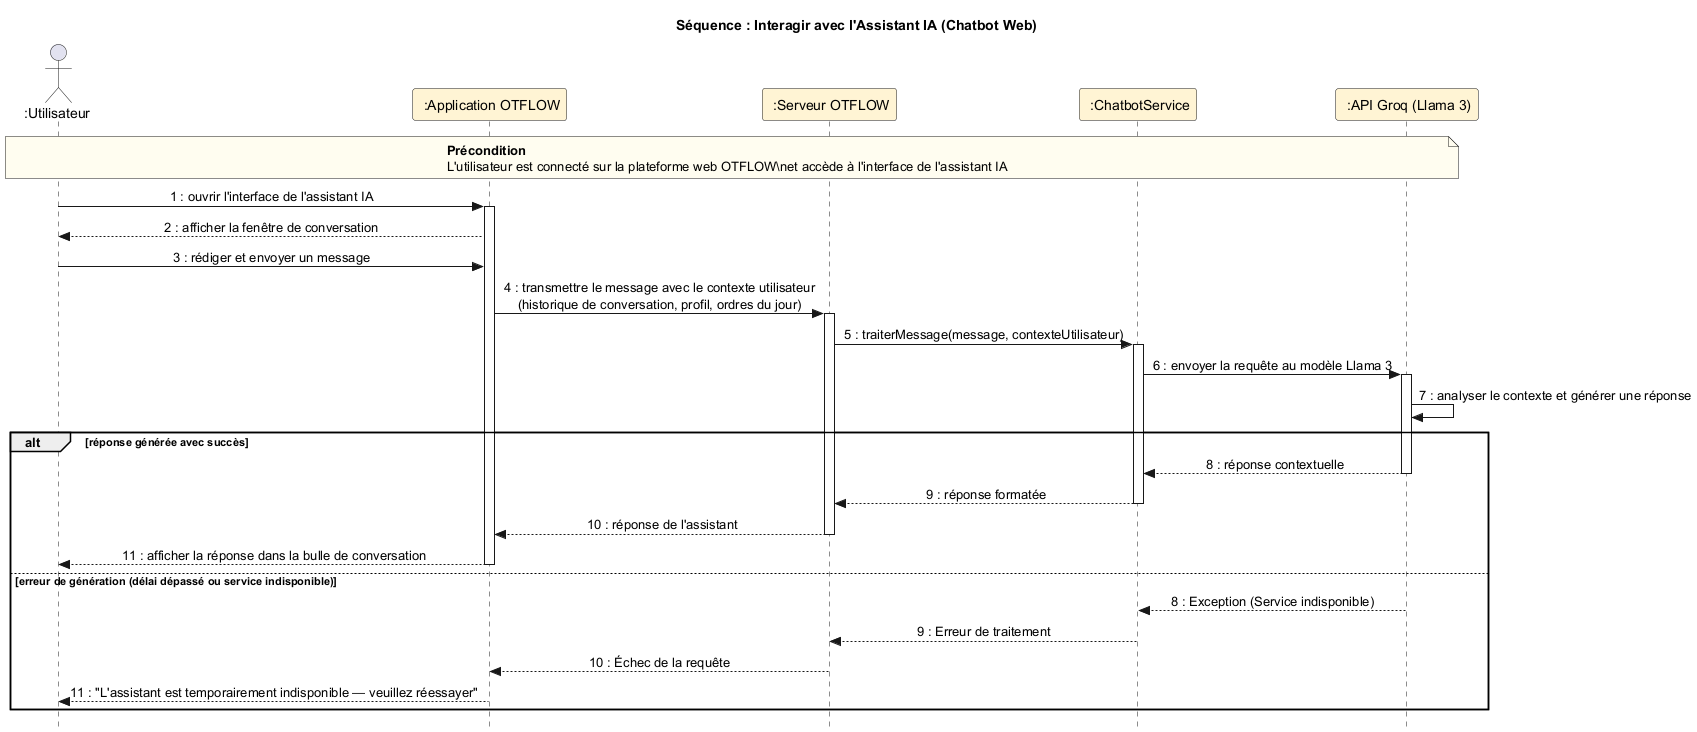
\includegraphics[width=0.85\textwidth, keepaspectratio]{sd_chatbot.png}
\caption{Diagramme de séquence -- Chatbot IA (Groq / Llama 3)}
\end{figure}

\subsection{Consultation du tableau de bord analytique}
L'utilisateur accède au tableau de bord. Le frontend envoie une requête au backend, qui agrège les données (nombre d'ordres, statuts, délais) et les retourne. Les graphiques se rafraîchissent automatiquement toutes les 30 secondes via un mécanisme de polling transparent.

\begin{figure}[H]
\centering
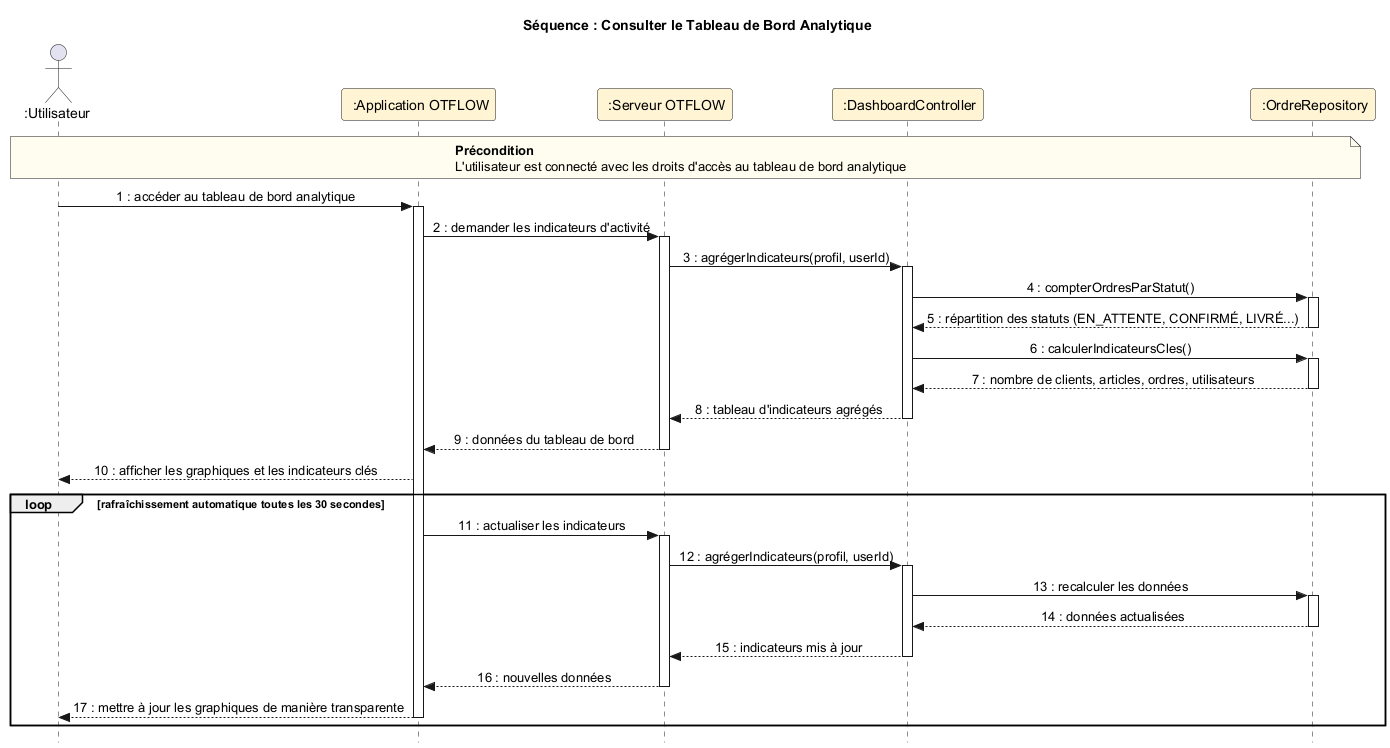
\includegraphics[width=0.85\textwidth, keepaspectratio]{sd_dashboard.png}
\caption{Diagramme de séquence -- Tableau de bord analytique (Polling Auto)}
\end{figure}

\subsection{Intelligence Artificielle sur Mobile (Génération de Rappels)}
L'assistant IA est également disponible sur l'application mobile. Le système analyse les réponses de l'IA (via Regex) pour y détecter des confirmations de rappels, puis synchronise de manière autonome ces rappels dans le stockage local natif de l'appareil (LocalStorage / Capacitor).

\begin{figure}[H]
\centering
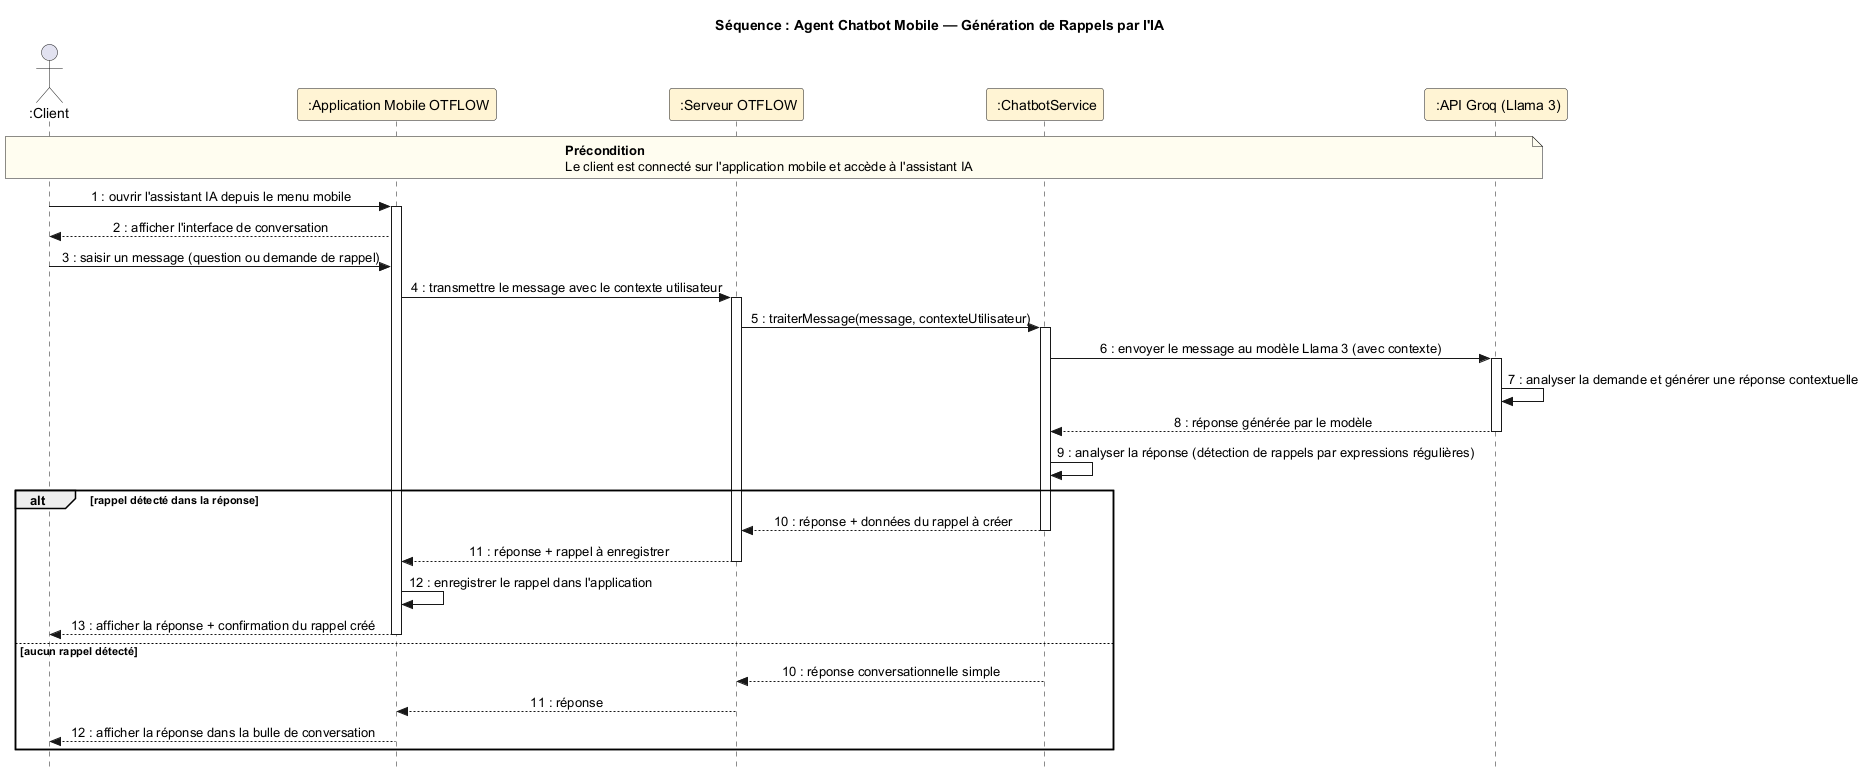
\includegraphics[width=0.85\textwidth, keepaspectratio]{sd_chatbot_mobile.png}
\caption{Diagramme de séquence -- Agent Chatbot Mobile (Génération de Rappels IA)}
\end{figure}

\section{Réalisation}

\subsection{Tableau de bord principal}
Le tableau de bord offre une vue synthétique de l'activité : nombre de clients, d'articles, d'ordres et d'utilisateurs, accompagnés de graphiques sur la répartition des statuts. Les données se rafraîchissent automatiquement toutes les 30 secondes.

\begin{figure}[H]
\centering
\includegraphics[width=0.75\linewidth]{TabBord2.png}
\caption{Tableau de bord principal dynamique}
\end{figure}

\begin{figure}[H]
\centering
\includegraphics[width=0.75\linewidth]{abBord.png}
\caption{Vue complémentaire du tableau de bord -- indicateurs clés}
\end{figure}

\subsection{Assistant IA Lumière -- Interface Web}
L'agent conversationnel propulsé par \textbf{Llama 3} via l'\textbf{API Groq} répond aux questions sur les commandes et livraisons, oriente les utilisateurs dans la navigation et assiste la création de nouveaux ordres. Le modèle Llama 3 via Groq garantit des temps de réponse très rapides et une bonne compréhension du français.

\begin{figure}[H]
\centering
\includegraphics[width=0.75\linewidth]{chatbot.png}
\caption{Interface de l'assistant IA Lumière (web)}
\end{figure}

\subsection{Assistant IA Lumière -- Interface Mobile}

\begin{figure}[H]
\centering
\includegraphics[width=4cm, height=7cm, keepaspectratio]{page_chatbot_mobile.png}
\caption{Interface conversationnelle de l'assistant IA Lumière (Llama 3 via API Groq) -- mobile}
\end{figure}

\section{Tests}

\begin{table}[H]
\centering
\caption{Résultats des tests -- Sprint 5}
\begin{tabular}{|p{8.5cm}|c|}
\hline
\textbf{Fonctionnalité testée} & \textbf{Résultat} \\
\hline
Chatbot IA -- réponses contextuelles (Llama 3) & Validé \\
\hline
Consultation des ordres via le chatbot & Validé \\
\hline
Tableau de bord -- rafraîchissement automatique & Validé \\
\hline
Graphiques de répartition des statuts & Validé \\
\hline
Chatbot mobile -- intégration API Groq & Validé \\
\hline
\end{tabular}
\end{table}

\section{Conclusion}
Le Sprint 5 complète la plateforme OTFLOW avec l'assistant IA Llama 3 via Groq, disponible sur web et mobile, et le tableau de bord analytique. Ces deux fonctionnalités renforcent l'autonomie des utilisateurs et la capacité de pilotage de l'activité logistique.

% =================================================
\chapter*{Conclusion Générale}
\addcontentsline{toc}{chapter}{Conclusion Générale}

Ce projet de fin d'études a abouti au développement complet de la plateforme \textbf{OTFLOW}, solution de gestion et de suivi des ordres de transport pour Lumière Transports. En centralisant l'information provenant de trois systèmes hétérogènes -- le TMS, le système Mobilité Lumière et le GPS Rimtrack -- OTFLOW répond aux problématiques identifiées et modernise les processus opérationnels de l'entreprise.

La sécurité du système repose sur une authentification JWT et un contrôle d'accès granulaire par permissions, garantissant l'isolation des données entre les acteurs. L'intégration du chatbot Llama 3 via l'API Groq constitue une valeur ajoutée significative, offrant une assistance contextuelle et réactive sur web et mobile. La méthodologie Agile Scrum, organisée en cinq sprints progressifs, a permis une livraison structurée et une validation continue avec l'entreprise d'accueil.

% =================================================
\chapter*{Bibliographie}
\addcontentsline{toc}{chapter}{Bibliographie}

\begin{thebibliography}{9}

\bibitem{scrum}
K. Schwaber et J. Sutherland, \textit{The Scrum Guide}, 2020.

\bibitem{springboot}
C. Walls, \textit{Spring Boot in Action}, Manning Publications.

\bibitem{angular}
Google, \textit{Angular Documentation}, \url{https://angular.io/docs}.

\bibitem{ionic}
Ionic Team, \textit{Ionic Framework Documentation}, \url{https://ionicframework.com/docs}.

\bibitem{mysql}
Oracle, \textit{MySQL Documentation}, \url{https://dev.mysql.com/doc}.

\bibitem{jwt}
Auth0, \textit{Introduction to JSON Web Tokens}, \url{https://jwt.io/introduction}.

\bibitem{groq}
Groq Inc., \textit{Groq API Documentation}, \url{https://console.groq.com/docs}.

\bibitem{leaflet}
Leaflet Contributors, \textit{Leaflet -- a JavaScript library for interactive maps}, \url{https://leafletjs.com}.

\bibitem{androidstudio}
Google, \textit{Android Studio Documentation}, \url{https://developer.android.com/studio}.

\end{thebibliography}

\end{document}
